\documentclass[a4paper,12pt]{article}

% 页面设置
\usepackage[top=2.54cm, bottom=2.54cm, left=3.17cm, right=3.17cm]{geometry}
\usepackage{fancyhdr}
\usepackage{ctex}
\usepackage{setspace}
\usepackage{graphicx}
\usepackage{times}
\usepackage{float}

% 页眉页脚设置
\pagestyle{fancy}
\fancyhf{}
\fancyhead[C]{\songti\zihao{-5}中央民族大学2026年大学生暑期社会实践成果}
\fancyfoot[C]{\thepage}
\renewcommand{\headrulewidth}{0.4pt}
\setlength{\headheight}{15pt}
\setlength{\headsep}{1.5cm}
\setlength{\footskip}{1.75cm}

% 行距设置 - 固定值22磅
\usepackage{setspace}
\setlength{\baselineskip}{22pt}
\setlength{\lineskip}{0pt}
\setlength{\lineskiplimit}{0pt}

% 字体设置
\setCJKmainfont{SimSun}

% 图片路径
\graphicspath{{./团队报告照片/}}

\begin{document}

% 标题
\begin{center}
\songti\zihao{3}\textbf{铭记烽火 赓续红色初心}
\end{center}
\begin{flushright}
\songti\zihao{3}——中国人民抗日战争纪念馆暑期社会实践调研报告
\end{flushright}

% 标题与摘要之间空一行（22磅）
\vspace{22pt}

% 摘要
\noindent\heiti\zihao{-4}\textbf{摘\quad\quad 要：}\songti\zihao{-4}\hspace{1em}本次暑期社会实践活动由刘佳鹏、安良玉、王冲三名成员组成的"赴北京市丰台区铭记烽火赓续红色初心调研实践团"，于2026年8月20日前往位于北京市丰台区卢沟桥城内街的中国人民抗日战争纪念馆开展为期3小时的深度实地调研学习。团队采用分工协作模式，安良玉负责第2展区日本侵华暴行板块的调研，刘佳鹏负责第3展区全民族抗战中流砥柱板块，王冲负责第4展区正面战场英勇抗战板块，并共同学习第5展区抗战胜利与历史启示内容。通过实地参观历史文物、观看影像资料、记录展陈内容、拍摄实践照片，团队系统学习了从九一八事变到抗战全面胜利的十四年抗战历史进程，深刻感受到中华民族不畏强暴、英勇抗争、团结奋斗的伟大抗战精神。本次实践活动增强了团队成员的历史责任感和民族自豪感，对培养爱国主义情怀、传承红色基因、提升综合实践能力具有重要意义。

% 摘要与关键词之间空一行（22磅）
\vspace{22pt}

% 关键词
\noindent\heiti\zihao{-4}\textbf{关键词：}\songti\zihao{-4}\hspace{1em}抗日战争；纪念馆；暑期实践；爱国主义教育；红色传承；团队协作

% 关键词与正文之间空一行（22磅）
\vspace{22pt}

% 正文
\songti\zihao{5}
\setlength{\parindent}{2em}
% 正文固定行距22磅
\linespread{1.0}
\selectfont

\section*{\songti\zihao{-3}\textbf{一、实践背景与目的}}

中国人民抗日战争是近代以来中国人民反抗外敌入侵第一次取得完全胜利的民族解放战争，是中华民族由衰败走向振兴的重大转折点。2026年是中国人民抗日战争暨世界反法西斯战争胜利81周年，回顾这段波澜壮阔的历史，对于当代青年学生铭记历史、珍爱和平、开创未来具有极其重要的现实意义。

为深入学习贯彻习近平新时代中国特色社会主义思想，传承红色基因，弘扬伟大抗战精神，我们"赴北京市丰台区铭记烽火赓续红色初心调研实践团"在指导教师张天华老师的指导下，于2026年暑期前往中国人民抗日战争纪念馆开展社会实践活动。中国人民抗日战争纪念馆位于北京市丰台区卢沟桥城内街，是全国唯一一座全面反映中国人民抗日战争历史的大型综合性专题纪念馆，是全国重要的爱国主义教育示范基地。

本次实践活动的背景深刻而紧迫。当今社会信息繁杂，部分青年对革命历史认知较为碎片化、表面化，缺少亲身沉浸式的历史体验。单纯依靠课堂理论学习难以真正体悟历史的厚重，因此，我们三人实践小组选择走进红色教育基地，通过实地走访、亲眼观察、现场调研的方式直面历史，弥补书本学习的不足，让红色教育从被动听课变为主动感悟、亲身实践。

本次实践活动的主要目的在于：第一，通过实地参观学习，深入了解中国人民抗日战争的历史进程和伟大意义，全面认识十四年抗战从局部抗战到全民族抗战的发展脉络；第二，通过观看历史文物和影像资料，直观感受革命先烈英勇抗战的光辉事迹，学习中国共产党在全民族抗战中发挥的中流砥柱作用；第三，通过团队学习交流，增强历史责任感和使命感，坚定理想信念，深刻认识今日和平生活来之不易；第四，通过撰写调研报告，系统总结学习成果，提升理论素养和实践能力，锤炼个人品德修养；第五，通过分工协作完成调研任务，培养团队协作精神、社会观察能力与实践创新能力。

立足当下，民族复兴任务艰巨、时代发展日新月异，青年更需要从抗战历史中汲取奋进力量，把爱国热情转化为学习动力，将个人理想融入国家发展，以青春之力担当新时代使命。

\section*{\songti\zihao{-3}\textbf{二、实践准备与组织实施}}

\subsection*{\songti\zihao{4}\textbf{（一）前期准备工作}}

为确保本次实践活动顺利开展并取得实效，团队在活动开展前进行了充分的准备工作。首先，全体组员自主查阅抗战历史资料，通过阅读《中国抗日战争史》《中国共产党历史》等权威著作，观看《伟大胜利 历史贡献》等纪录片，系统学习抗日战争的历史背景、重大事件、重要人物和深远影响，为实地调研奠定扎实的理论基础。

其次，团队成员通过中国人民抗日战争纪念馆官方网站和公众号，熟悉场馆布局、展陈内容与重点史实，确定调研方向和重点关注内容。根据场馆展览布局和团队成员特长，我们确定了明确的分工方案：王冲担任团队总负责人，统筹行程安排、纪律管理与安全保障；安良玉负责第2展区日本侵华暴行板块的深度调研与文字记录；刘佳鹏负责第3展区全民族抗战中流砥柱板块的学习整理；王冲负责第4展区正面战场英勇抗战板块的资料收集；摄影工作由三人共同完成，确保每个展区都有充分的影像记录。

再次，团队完成了场馆实名预约，熟知参观规则与拍摄要求。中国人民抗日战争纪念馆作为国家级纪念场馆，要求参观者提前实名预约、携带有效证件、着装得体、保持肃静、文明拍摄。团队成员认真学习参观须知，明确纪念馆内禁止喧哗、禁止触摸文物、禁止使用闪光灯等规定，确保在参观过程中展现当代大学生的良好素质。

最后，团队成员提前准备工具设备，检查手机、相机等设备的电量和存储空间，准备记录本、笔等文字记录工具。全员着装庄重整洁，端正实践态度，怀着崇敬之心准备开展这次意义深远的红色之旅。

\subsection*{\songti\zihao{4}\textbf{（二）实施过程}}

2026年8月20日上午，团队成员准时在学校集合，由负责人王冲重申活动纪律、安全事项与分工后统一出发，全程结伴行动。抵达中国人民抗日战争纪念馆后，我们首先在纪念馆正门合影留念。纪念馆正门墙面镶嵌金色馆名大字，大门上方悬挂红色横幅，文字为"铭记历史 缅怀先烈 珍爱和平 开创未来"，这十六个字正是我们此行的宗旨和初心。

\begin{figure}[H]
\centering
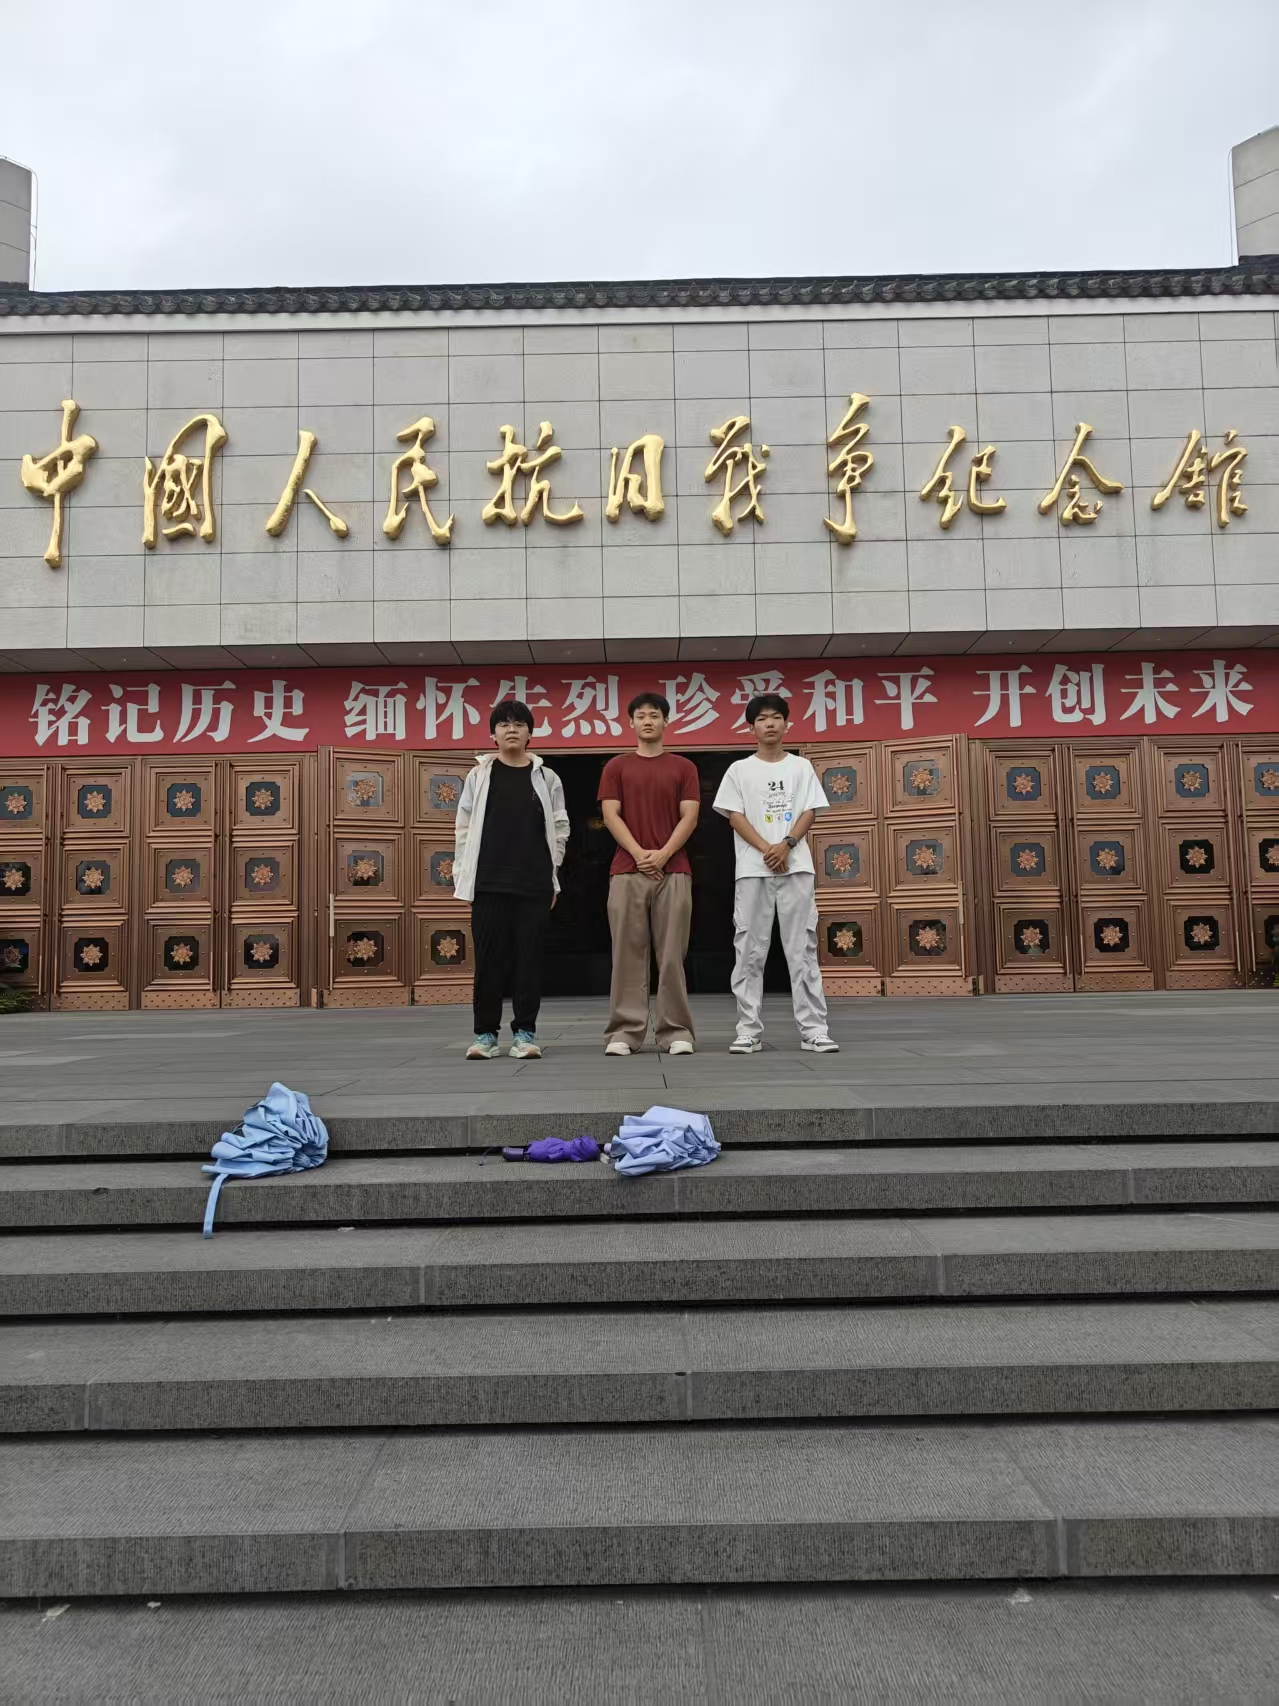
\includegraphics[width=0.7\textwidth]{A (1).jpg}
\caption{实践团队在中国人民抗日战争纪念馆正门合影}
\end{figure}

进入馆内后，我们首先参观了序厅的大型军民抗战浮雕。这幅青铜浮雕气势恢宏，雕刻了军人、工人、农民、学生等各阶层人物形象，展现了全民族万众一心投身抗日战争的壮阔场面。团队成员驻足凝视，深切感受到抗日战争是一场真正的人民战争，正是全体中华儿女的团结奋斗，才赢得了最终的胜利。

\begin{figure}[H]
\centering
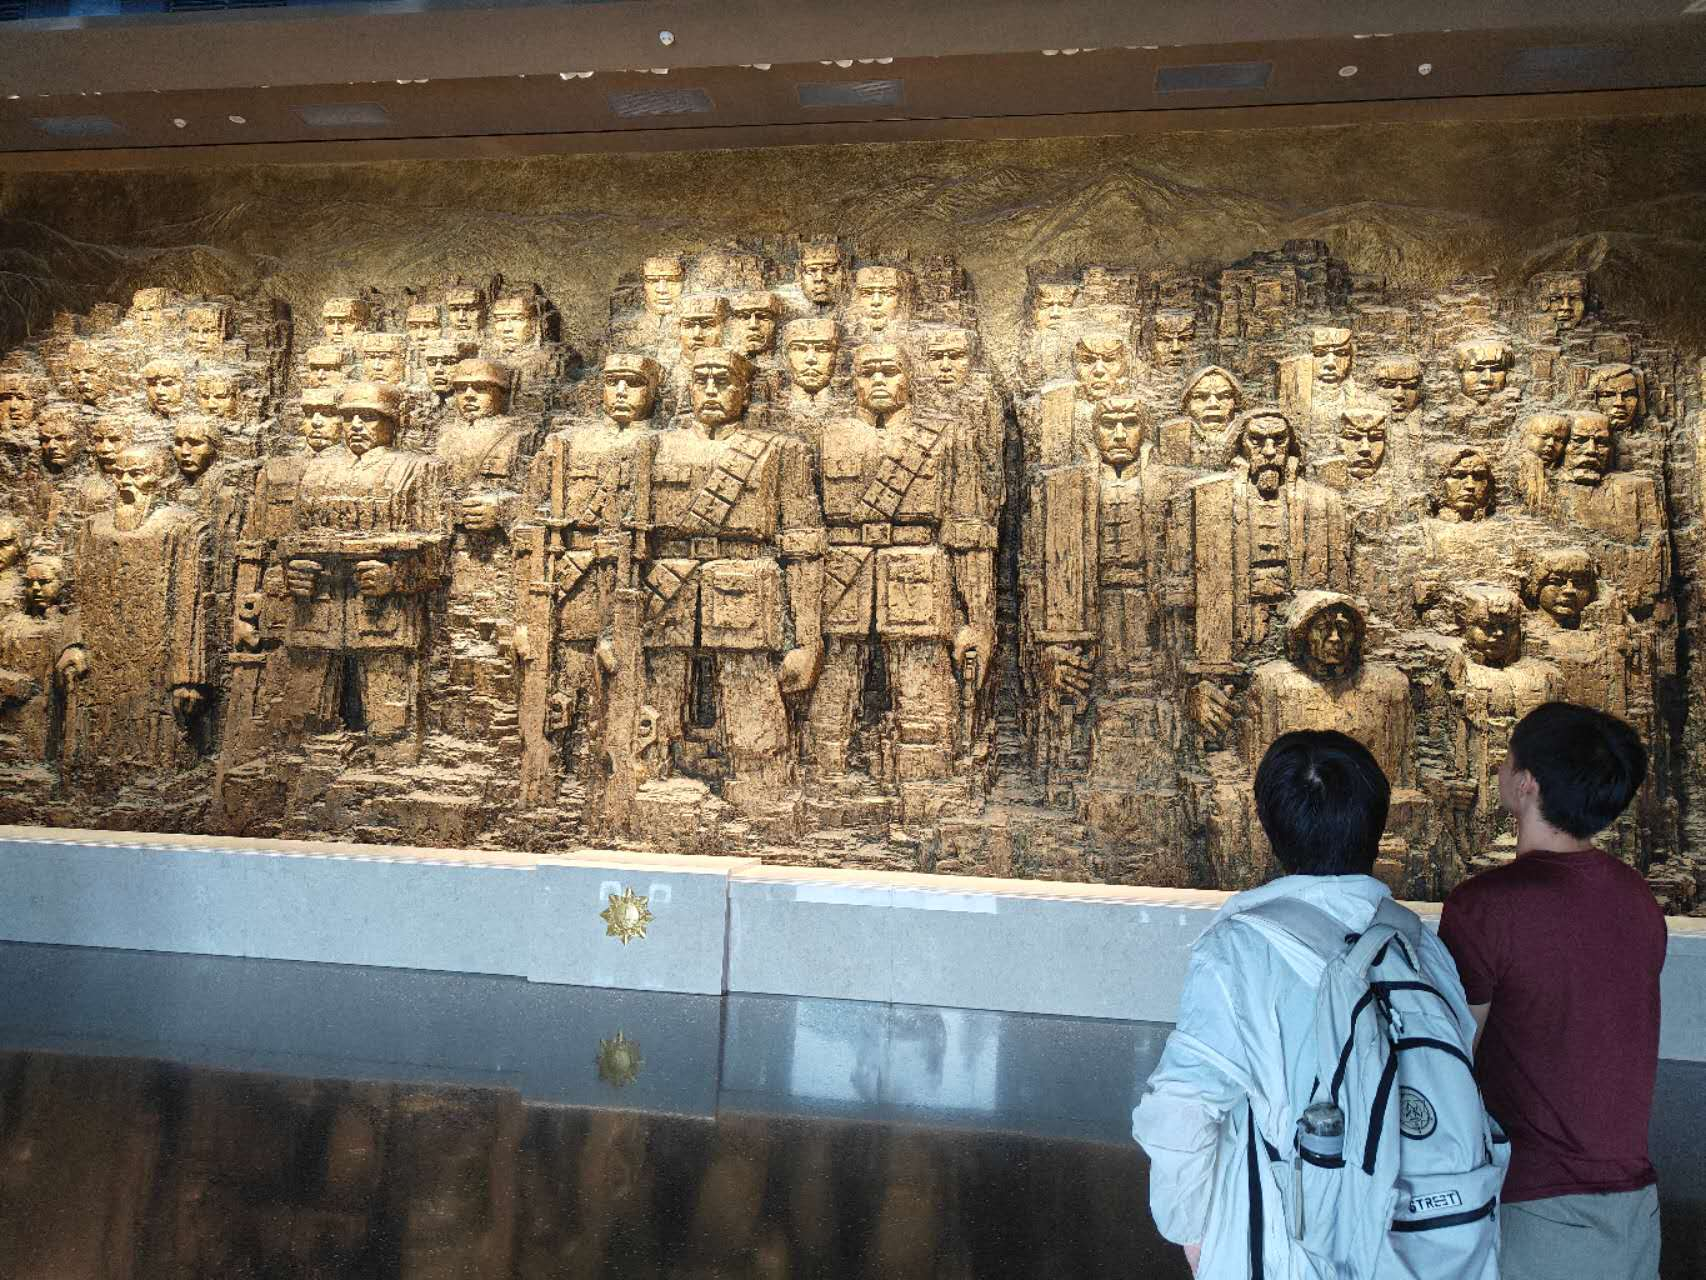
\includegraphics[width=0.7\textwidth]{A (2).jpg}
\caption{团队成员参观纪念馆大型军民抗战浮雕}
\end{figure}

随后，我们进入主展厅，映入眼帘的是"为了民族解放与世界和平"主题展墙。展墙红色大字标题醒目，副标题为"纪念中国人民抗日战争暨世界反法西斯战争胜利80周年主题展览"，墙面还有黄土高原浮雕、吹军号战士雕塑与延安宝塔山浮雕元素，点明本次展览核心主题，展现抗日战争不仅关乎中华民族解放，也属于世界反法西斯战争的重要组成部分。

\begin{figure}[H]
\centering
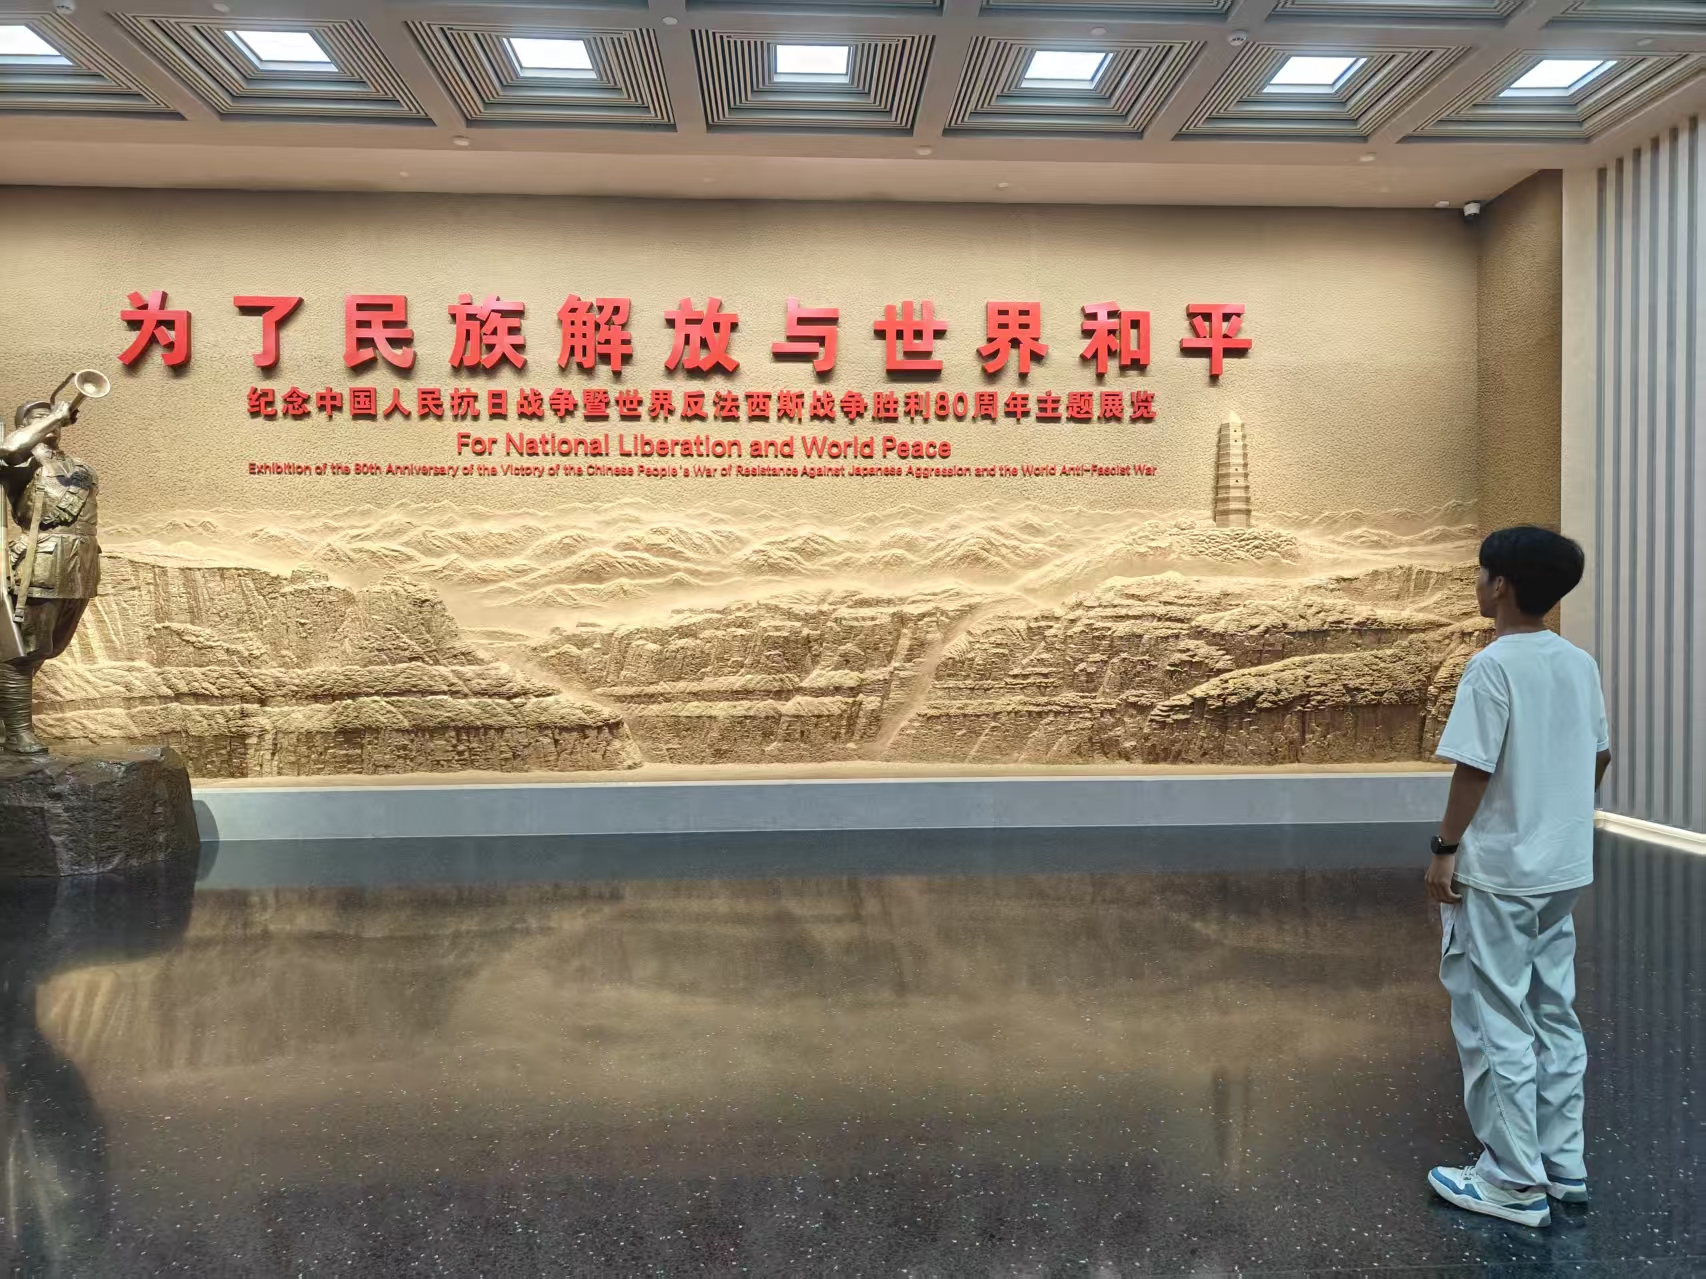
\includegraphics[width=0.7\textwidth]{A (4).jpg}
\caption{纪念抗战胜利80周年主题展览大厅}
\end{figure}

按照预定计划，团队成员分别前往各自负责的展区开展深度调研学习，同时保持沟通联系，确保活动安全有序进行。

\section*{\songti\zihao{-3}\textbf{三、第2展区：日本侵华暴行——历史的沉痛记忆}}

\subsection*{\songti\zihao{4}\textbf{（负责人：安良玉）}}

第2展区集中展示了日本侵略者在侵华战争期间犯下的滔天罪行，这是中华民族历史上最为沉痛的记忆。作为本板块的调研负责人，我怀着沉重的心情走进展厅，每一件展品、每一张照片、每一段文字都是对日本军国主义暴行的铁证，都是对中华民族苦难历史的真实记录。

展区开篇即展示了九一八事变后日本侵略军在东北的暴行。1931年9月18日，日本关东军悍然发动九一八事变，拉开了日本侵华战争的序幕。展区内陈列着大量历史照片和文献资料，记录了日本侵略军占领东北后实施的血腥统治：强占土地、掠夺资源、奴役劳工、镇压抗日力量。一张张被烧毁的村庄照片、一份份被掠夺资源的统计数据，无声地控诉着侵略者的罪恶。

展区重点展示了南京大屠杀这一惨绝人寰的暴行。1937年12月，日军攻占南京后，进行了长达六周的大规模屠杀、强奸、抢劫、纵火，30万中国同胞惨遭杀戮。展区内陈列的历史照片触目惊心：堆积如山的尸体、哭泣的幸存者、被烧毁的建筑。展柜中展出的幸存者证言、外国人士的记录、日军官兵的日记，从不同角度证实了这场人类历史上罕见的暴行。作为一名当代青年，站在这些历史证据面前，我深感震撼和悲痛，更加深刻地认识到和平的可贵。

展区还详细介绍了平顶山惨案、潘家峪惨案等一系列屠村事件。在"万人坑"复原场景前，我驻足良久，那些累累白骨无声地控诉着侵略者的残暴。解说牌介绍，仅在抚顺平顶山一地，日军就屠杀了3000多名无辜百姓，制造了震惊中外的平顶山惨案。类似的惨案在中国大地上不计其数，每一个数字背后都是一条鲜活的生命，都是一个破碎的家庭。

特别令人发指的是日军实施的"三光政策"——烧光、杀光、抢光。展区通过历史照片、实物证据和幸存者口述，详细记录了日军在华北敌后抗日根据地实施的疯狂扫荡。成片的村庄被烧毁，无数百姓被杀害，大量粮食和物资被抢劫一空。冀中地区、晋察冀边区、山东抗日根据地都遭受了惨重损失。中国人民在极其艰苦的条件下坚持抗战，付出了巨大的民族牺牲。

展区还专门设置了慰安妇制度罪行展示区。日军在侵华战争期间，强征大量中国、朝鲜等亚洲国家妇女充当"慰安妇"，这是对女性尊严的严重践踏，是反人类的罪行。展区展出的幸存者照片、证言材料、历史文献，揭露了这一罪恶制度的真相。看到那些饱经苦难的老人面容，我深感痛心，也更加坚定了维护历史真相、反对历史虚无主义的决心。

展区还揭露了日军进行的细菌战和毒气战罪行。臭名昭著的731部队在中国东北秘密研制细菌武器，用活人进行惨无人道的人体实验。展区展出的历史照片、实验设施模型、受害者资料，让人不寒而栗。日军还在战场上大量使用化学武器，违反国际公约，给中国军民造成严重伤亡。这些铁证如山的历史事实，充分揭露了日本军国主义的反人类本质。

通过对第2展区的深入学习，我深刻认识到：日本军国主义给中国人民带来了深重灾难，中华民族经历了前所未有的苦难。但是，再残暴的侵略也无法摧毁中国人民的抗战意志，反而激发了中华民族空前的团结和觉醒。铭记历史不是为了延续仇恨，而是为了警示后人珍爱和平、维护正义，坚决反对一切形式的侵略战争和法西斯主义。历史不容忘却，正义必将战胜邪恶。

\section*{\songti\zihao{-3}\textbf{四、第3展区：全民族抗战的中流砥柱——中国共产党的光辉历程}}

\subsection*{\songti\zihao{4}\textbf{（负责人：刘佳鹏）}}

第3展区生动展现了中国共产党在全民族抗战中发挥的中流砥柱作用，这是我负责调研的核心板块。通过深入学习，我深刻认识到，抗日战争的胜利，是中国共产党坚强领导的结果，是人民战争的伟大胜利。

展区开篇即展示了中国共产党率先举起武装抗日旗帜的历史。九一八事变爆发后，中国共产党立即发表宣言，号召全国人民奋起抵抗日本侵略。1931年9月20日，中共中央发表《关于日本帝国主义强占满洲事变的决议》，这是国内第一个号召武装抗日的宣言。在中国共产党领导下，东北抗日联军、东北义勇军等抗日武装力量迅速组建，在极其艰苦的条件下坚持抗战长达14年。

展区重点介绍了著名抗日爱国将领吉鸿昌烈士的英勇事迹。吉鸿昌将军坚决反对"不抵抗政策"，积极投身抗日救亡运动，最终为国捐躯。展柜中陈列着吉鸿昌烈士的肖像、历史照片和珍贵文物，最令人动容的是他就义前写下的《就义诗》："恨不抗日死，留作今日羞。国破尚如此，我何惜此头。"这首诗字字千钧，彰显了烈士宁死不屈的爱国气节和视死如归的革命精神。我在展板前久久驻足，深受震撼，这就是中国共产党人和爱国志士的崇高品格。

\begin{figure}[H]
\centering
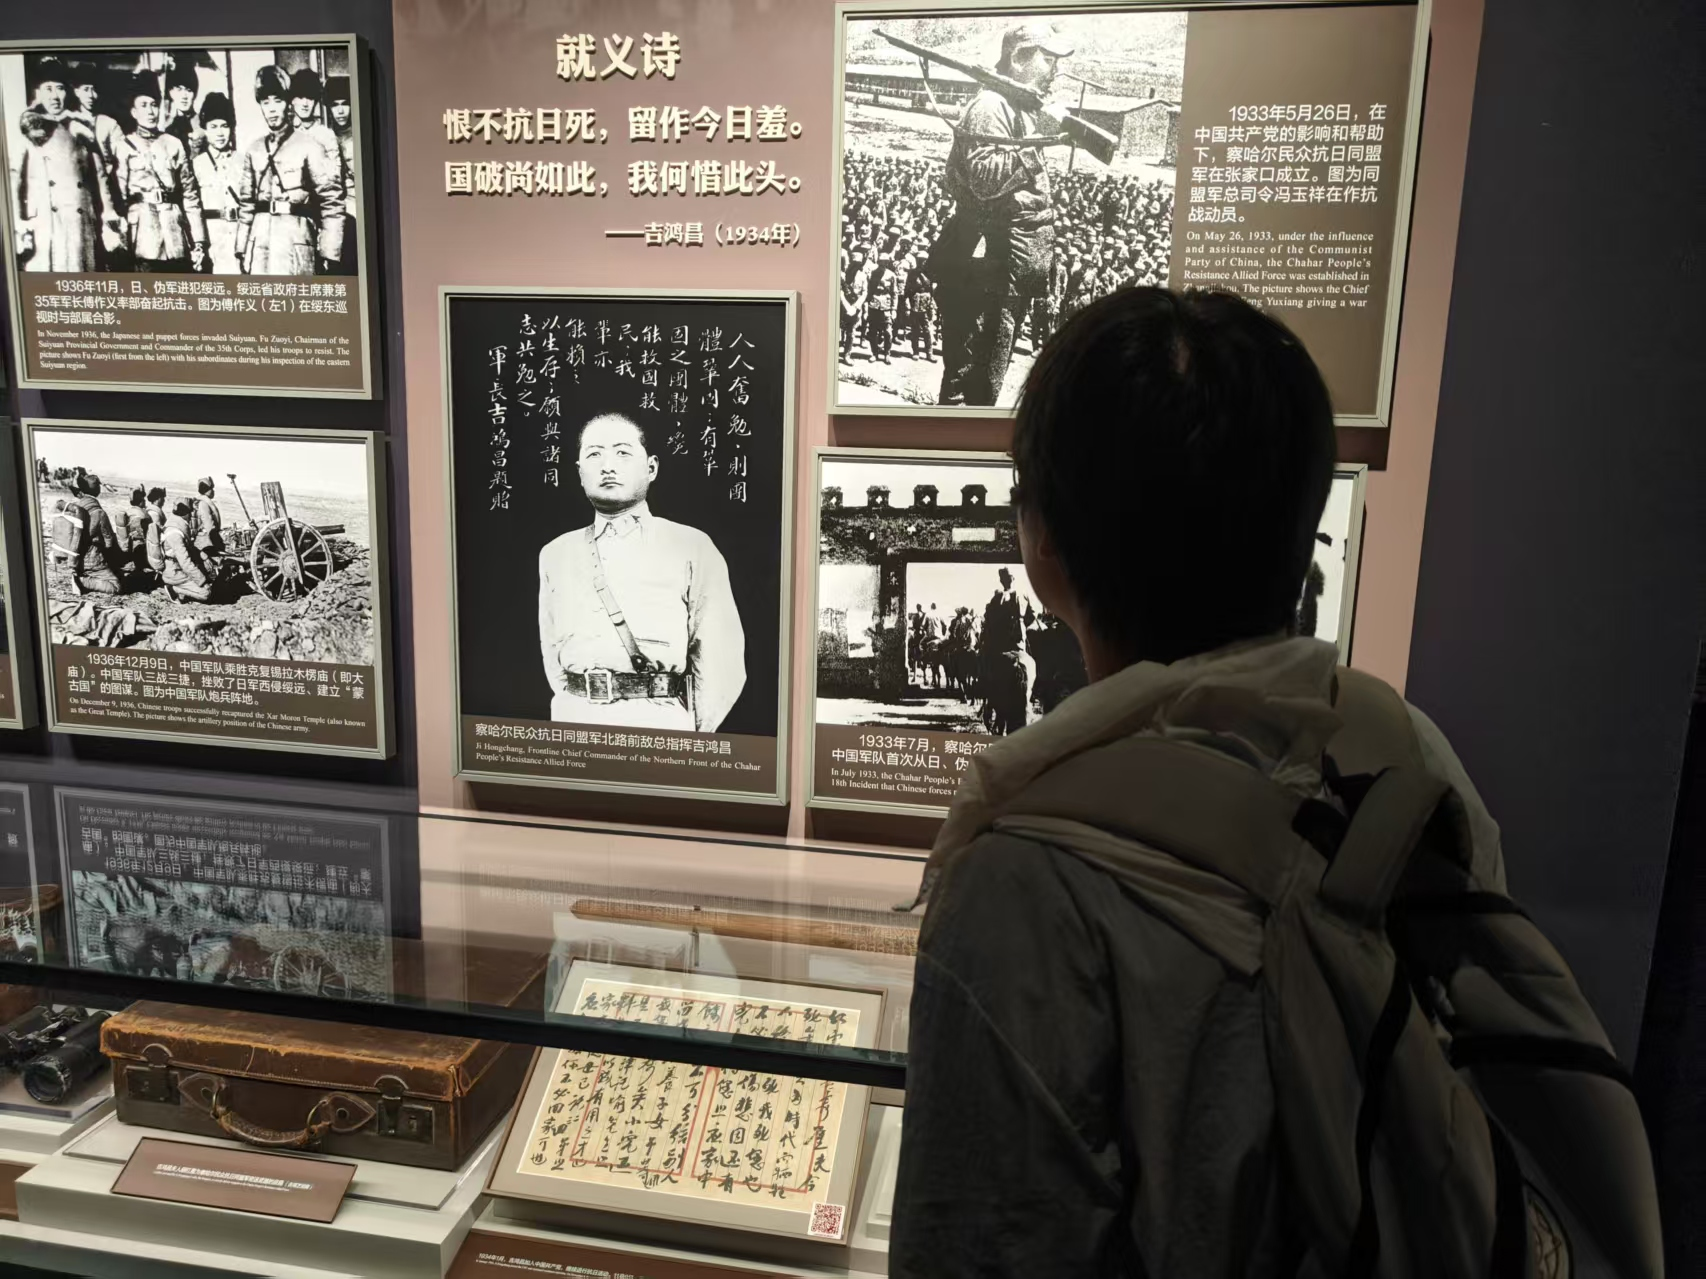
\includegraphics[width=0.7\textwidth]{A (5).jpg}
\caption{吉鸿昌烈士史料展区}
\end{figure}

展区详细介绍了一二九运动的历史意义。1935年12月9日，北平学生举行抗日救国示威游行，反对华北自治，要求停止内战、一致抗日。展区内的大型浮雕生动刻画了爱国青年学生高举标语横幅、游行示威的场景，浮雕上方引用毛泽东的评价："一二九运动是动员全民族抗战的运动，它准备了抗战的思想，准备了抗战的人心，准备了抗战的干部。"这场运动唤醒了广大民众的抗日意识，推动了抗日民族统一战线的形成。作为一名当代大学生，我深感青年在民族危亡时刻的历史责任，也更加坚定了为国家富强、民族复兴而奋斗的决心。

\begin{figure}[H]
\centering
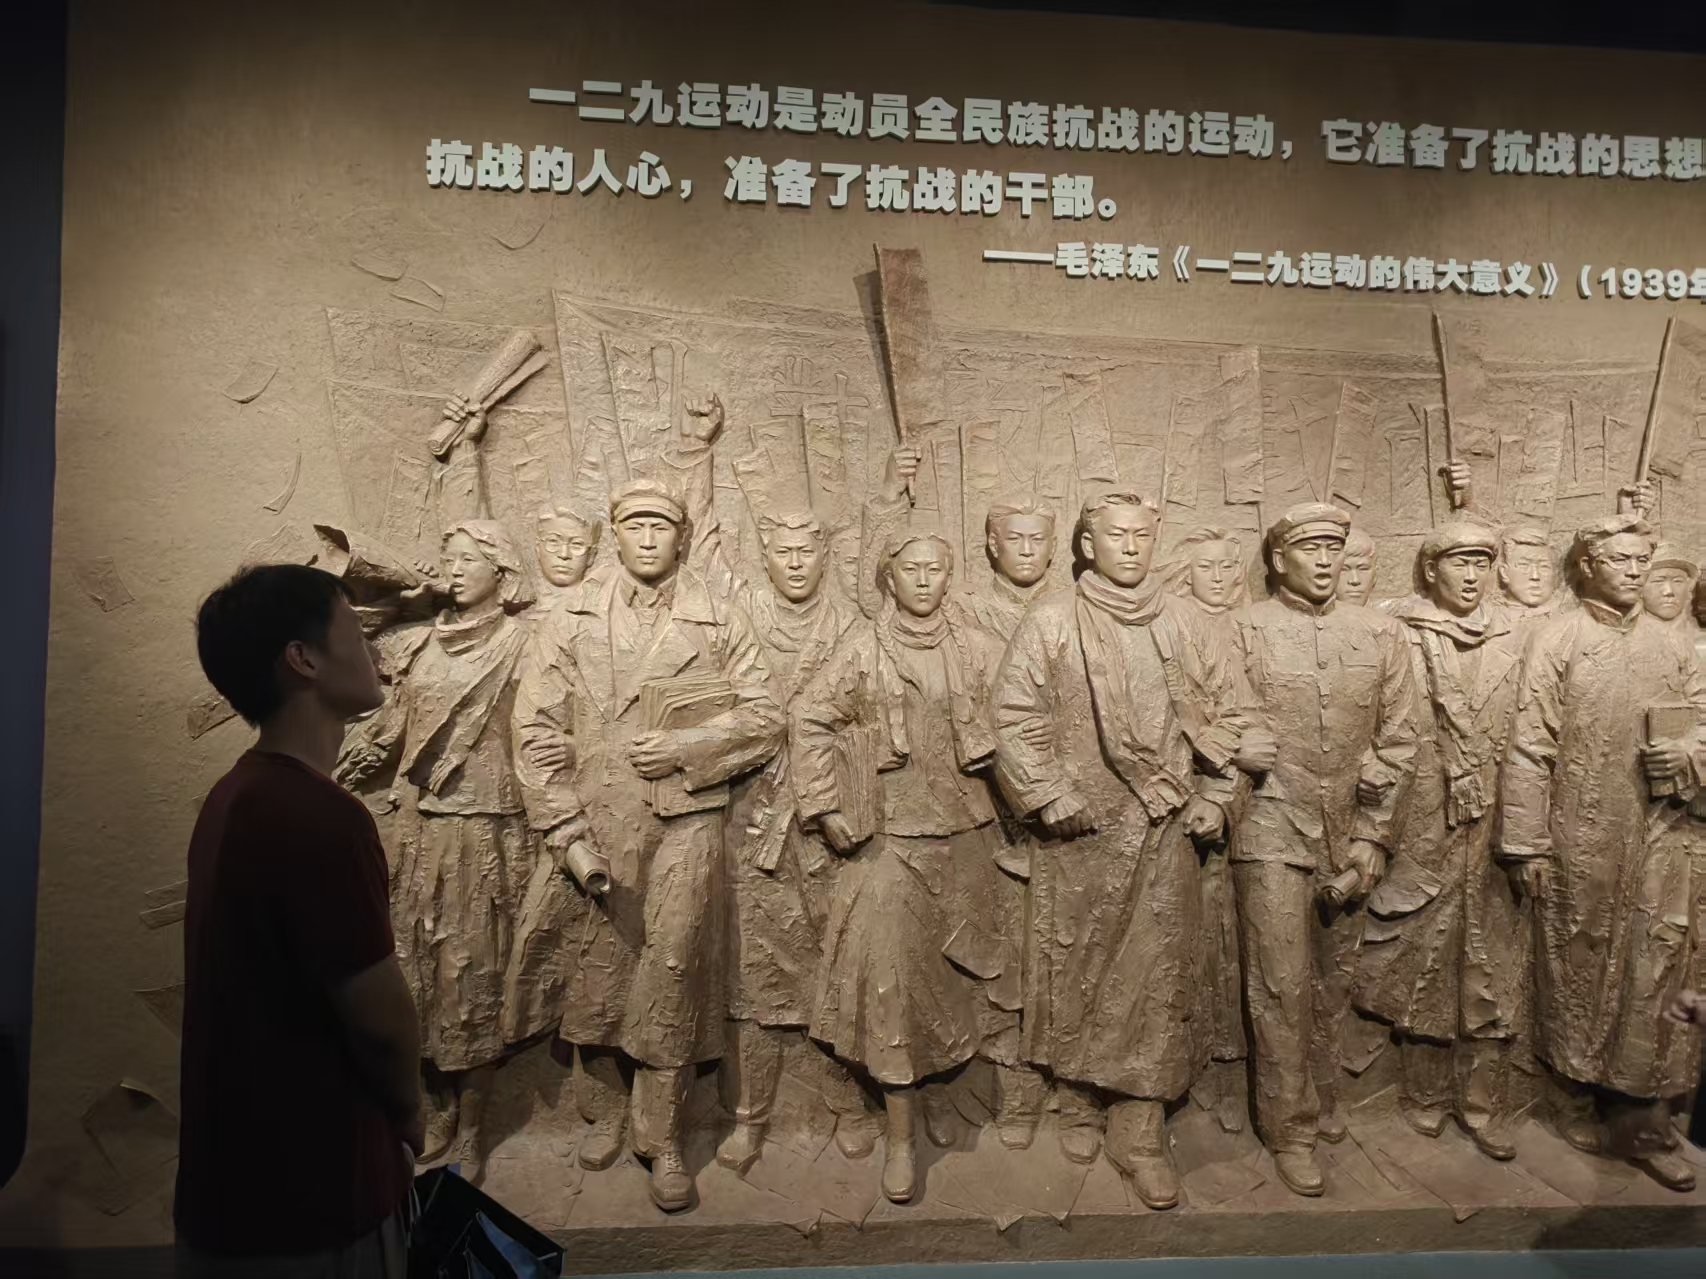
\includegraphics[width=0.7\textwidth]{A (6).jpg}
\caption{一二九运动浮雕展区}
\end{figure}

展区重点展示了中国共产党领导的敌后战场的英勇抗战。全面抗战爆发后，八路军、新四军挺进敌后，开辟抗日根据地，开展游击战争。展板介绍了八路军第115师的光辉战史，特别是平型关大捷这一全民族抗战爆发以来的首次大捷。1937年9月25日，八路军第115师在平型关伏击日军，歼敌1000余人,打破了日军不可战胜的神话，极大地振奋了全国军民的抗战信心。展柜中陈列着115师战士使用过的武器装备、缴获的日军物品、战斗记录等珍贵文物。

\begin{figure}[H]
\centering
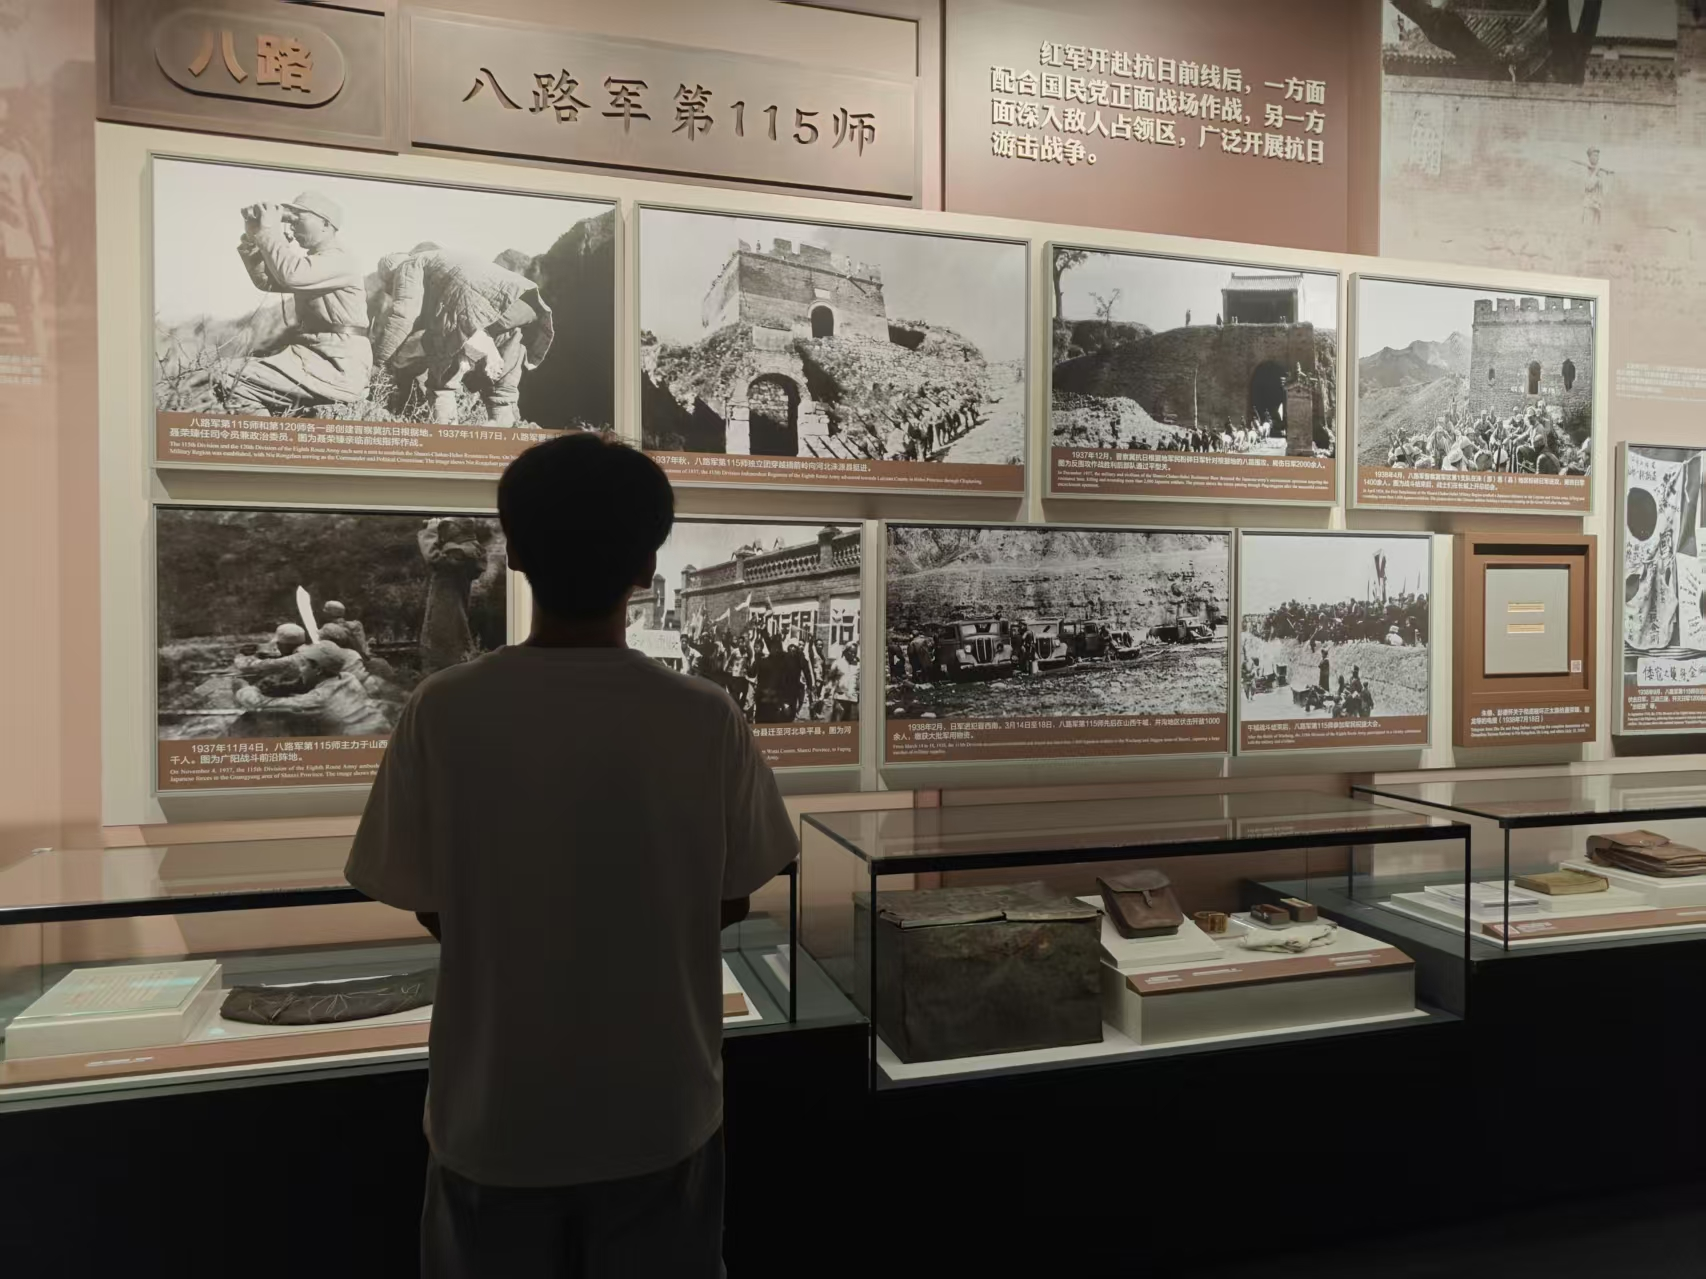
\includegraphics[width=0.7\textwidth]{A (7).jpg}
\caption{八路军115师史料展板}
\end{figure}

展区还通过实景复原技术，搭建了残垣断壁的战争场景，配合光影烟雾效果，直观还原了敌后战场残酷的巷战环境。展柜中陈列着当年的重机枪等武器文物。这个场景让我深切感受到，抗日战士就是在这样艰险的环境中，凭借顽强的意志和灵活的战术，与装备精良的日军展开殊死搏斗，用鲜血和生命保卫着祖国的每一寸土地。

\begin{figure}[H]
\centering
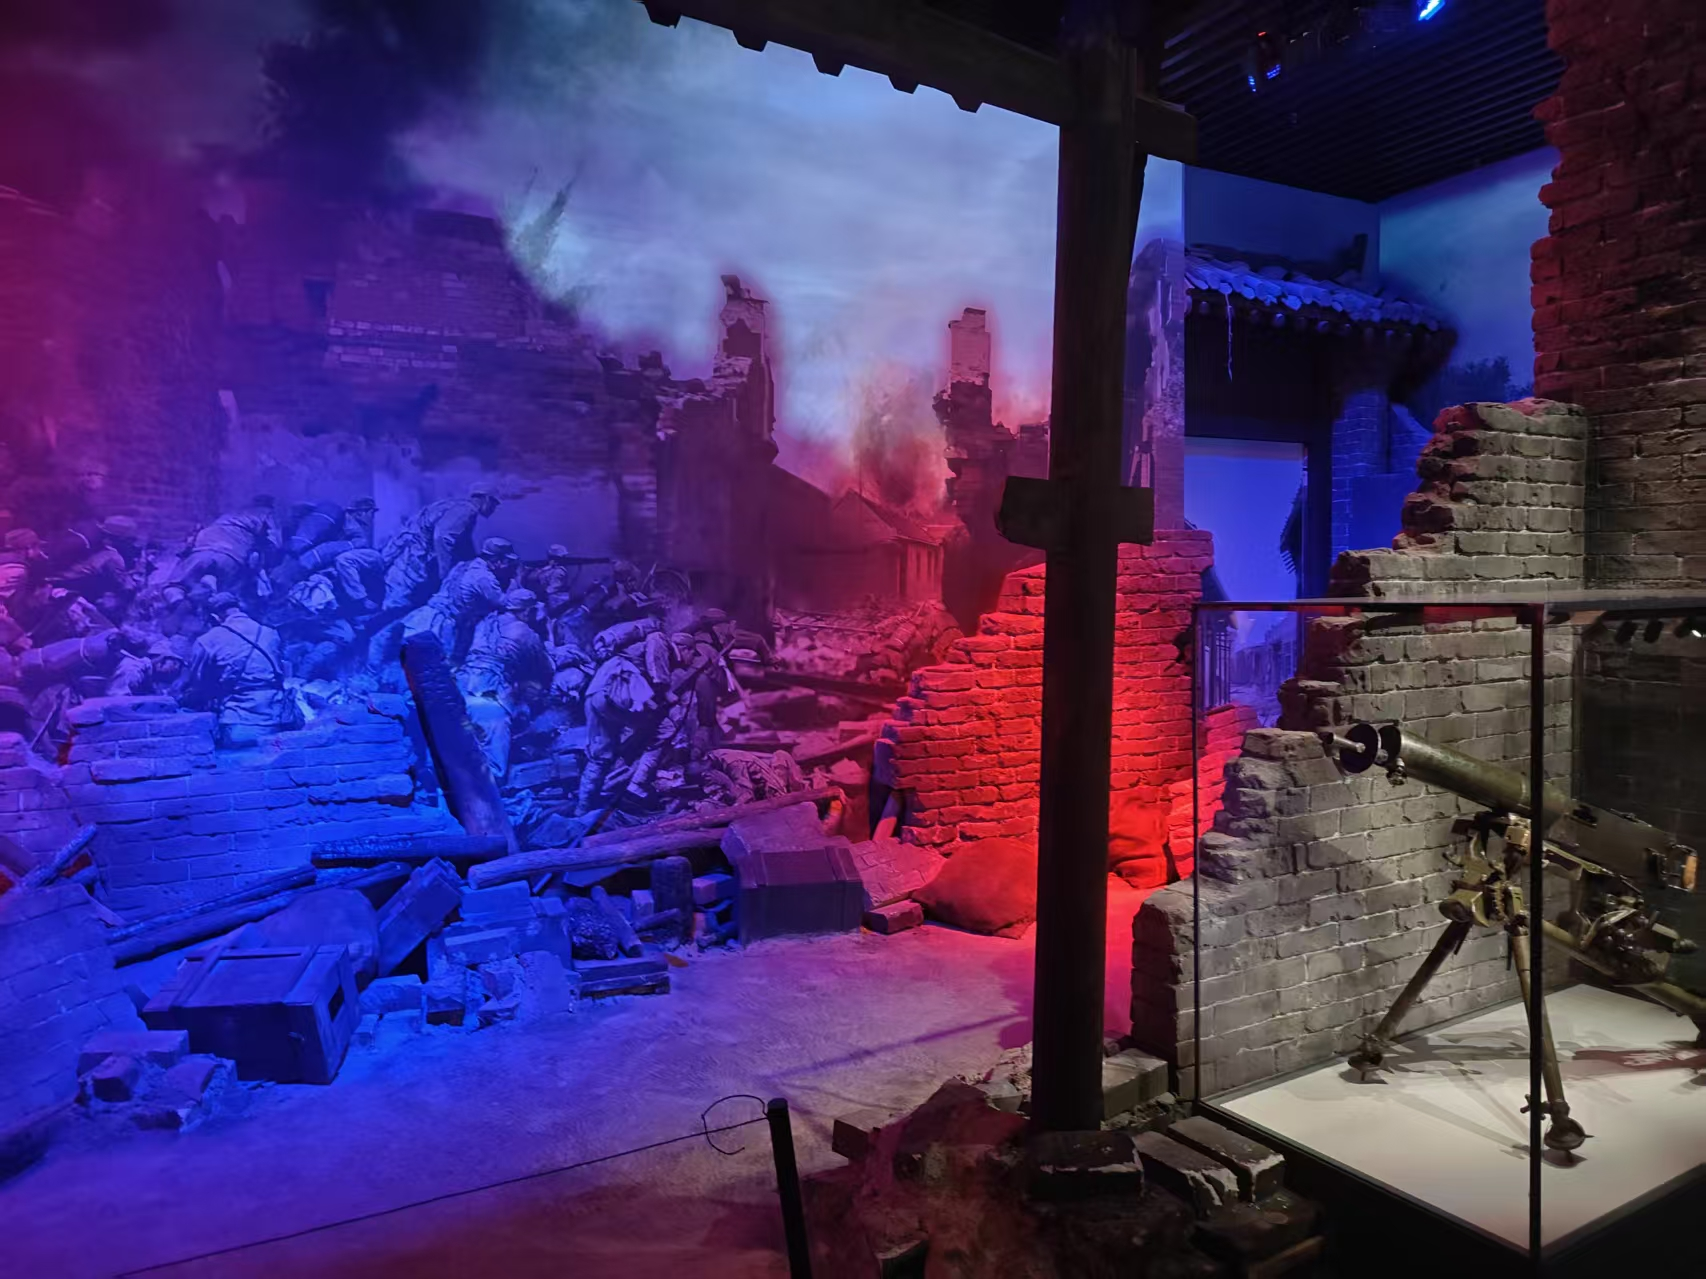
\includegraphics[width=0.7\textwidth]{A (8).jpg}
\caption{抗战巷战场景复原}
\end{figure}

展区特别设置了毛泽东军事思想展示区，重点介绍了《论持久战》和《抗日游击战争的战略问题》这两篇重要著作。1938年5月，毛泽东发表《论持久战》，科学分析了中日双方的基本特点，驳斥了"亡国论"和"速胜论"，系统阐述了持久抗战的战略方针，明确指出抗日战争将经历战略防御、战略相持、战略反攻三个阶段，最后胜利属于中国。展板上摘录的经典段落："抗日战争是持久战，最后胜利是中国的"，这一科学论断为全国抗战指明了方向，坚定了全国人民的抗战信心。

\begin{figure}[H]
\centering
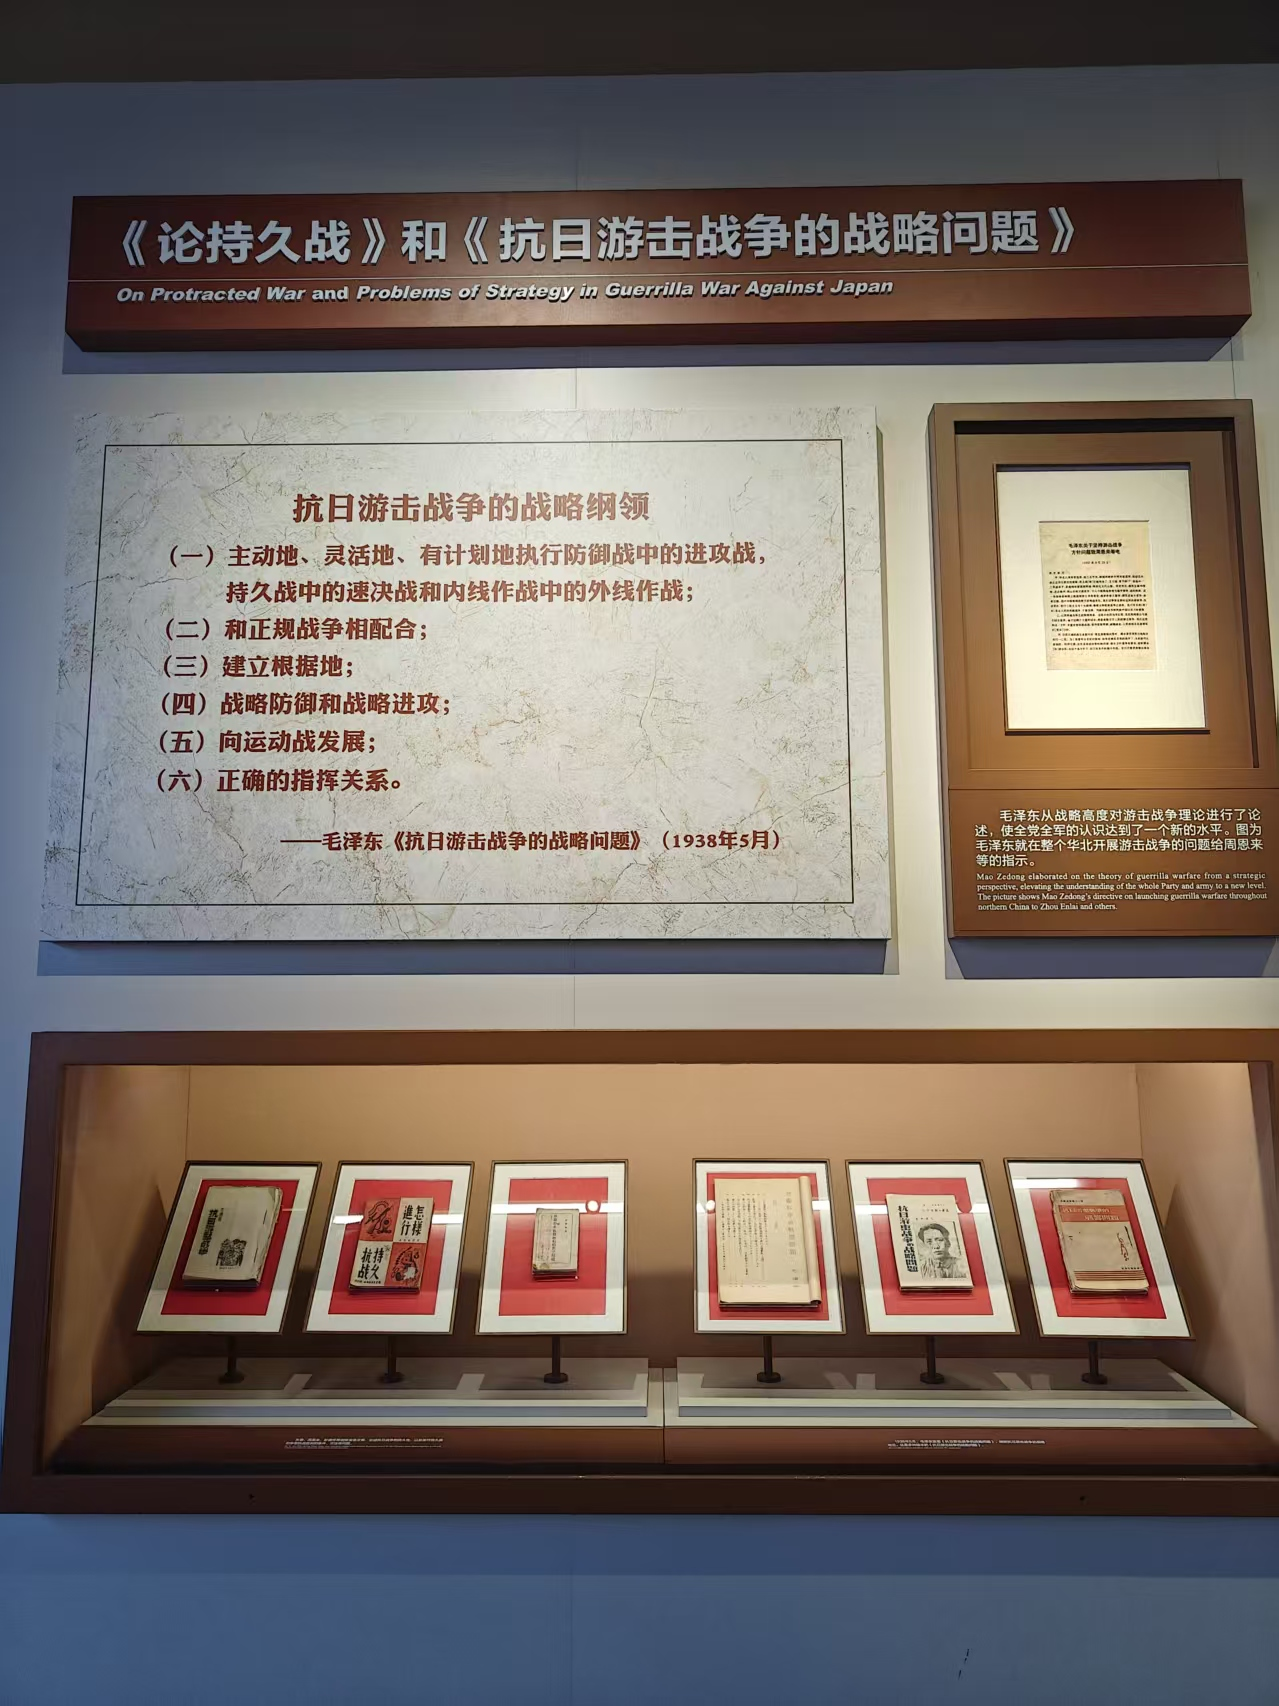
\includegraphics[width=0.7\textwidth]{A (9).jpg}
\caption{《论持久战》主题展板}
\end{figure}

\begin{figure}[H]
\centering
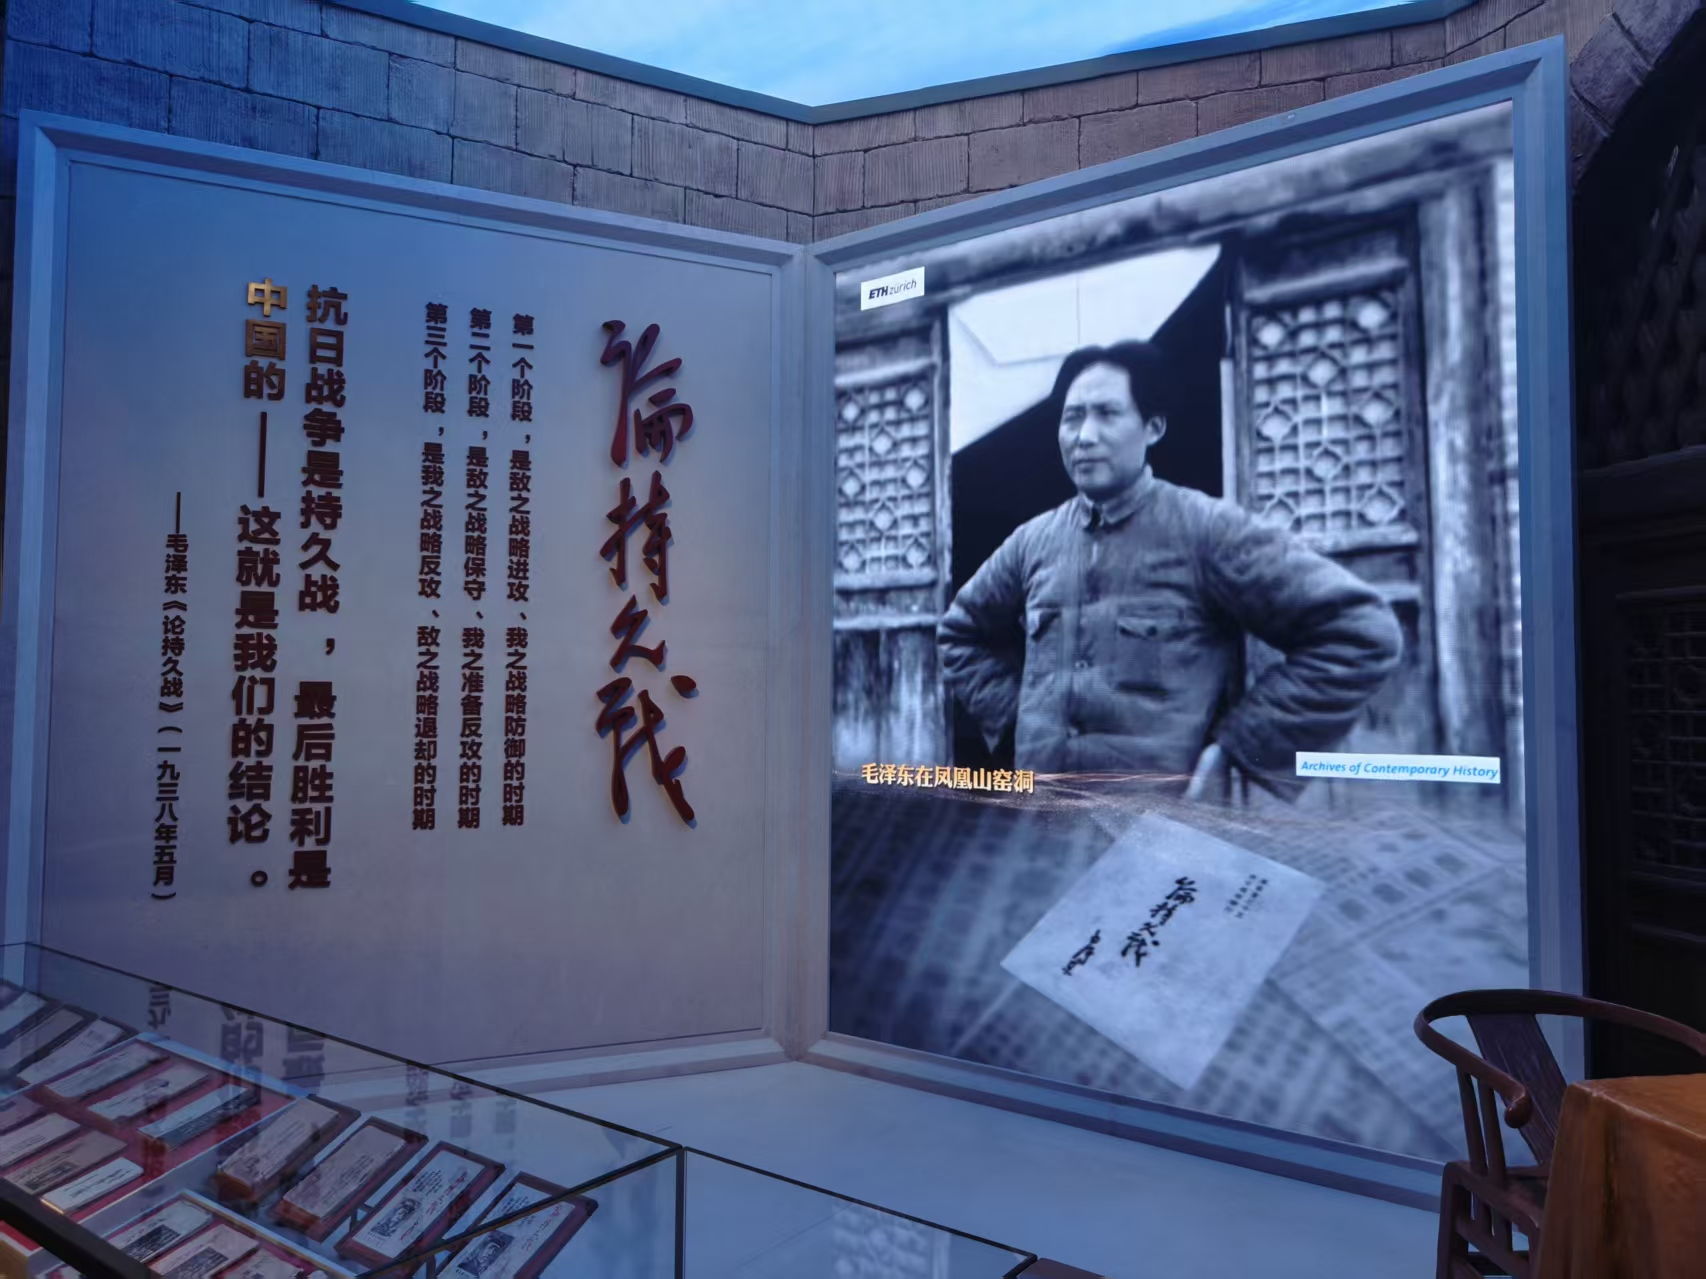
\includegraphics[width=0.7\textwidth]{A (10).jpg}
\caption{《论持久战》与《抗日游击战争的战略问题》展区}
\end{figure}

展区还介绍了延安作为抗战时期革命圣地的重要地位。在民族危亡之际，无数爱国青年和进步知识分子冲破封锁，奔赴延安，投身抗日救亡运动。展板展示了八路军驻陕办事处用车运送爱国青年北上延安的照片，引用了柯仲平1939年的诗作《延安与中国青年》，生动描绘了青年不惧艰苦、一心奔赴延安的热情。展区还展示了何干之、梁未闻、艾思奇等上海知名文化人士赴延安途中的合影。延安成为全国进步力量的汇聚地，为抗战和革命培养了大批干部人才。

\begin{figure}[H]
\centering
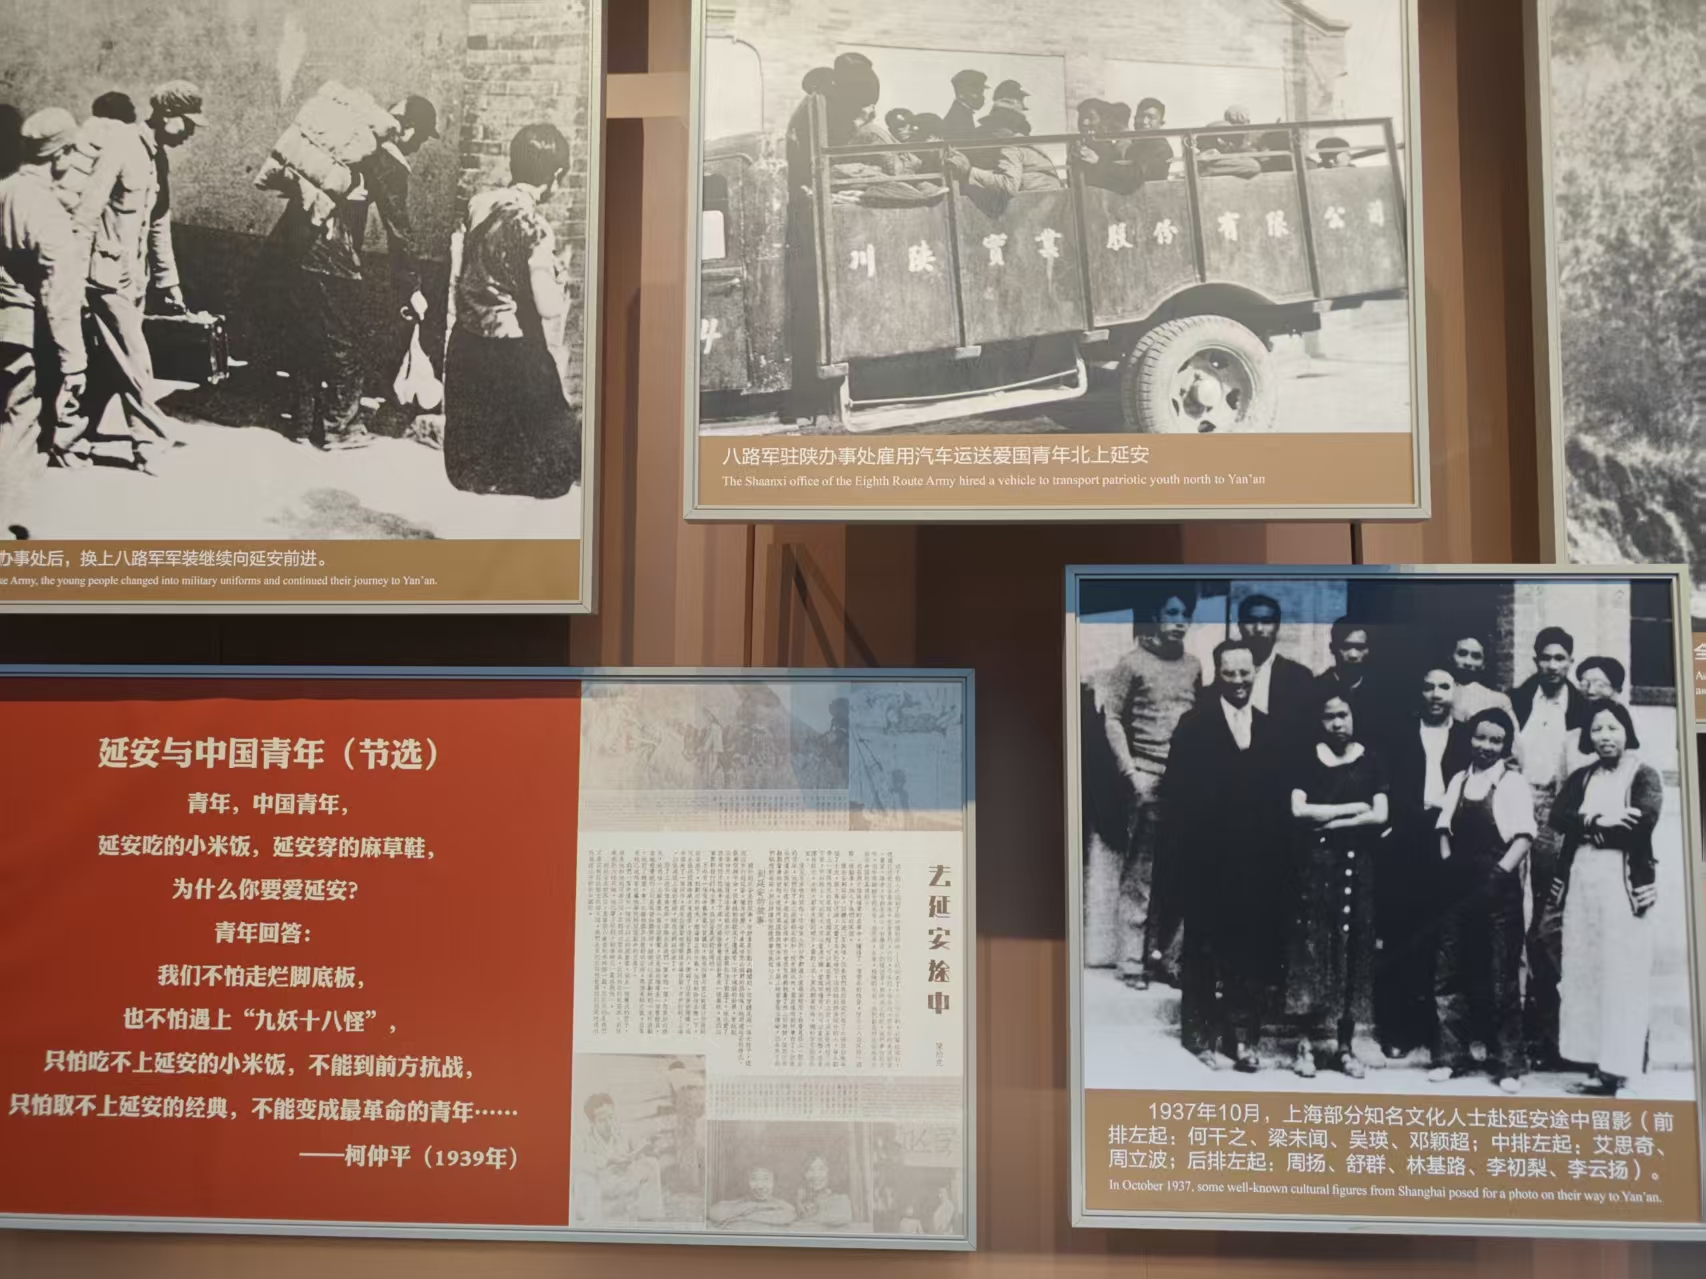
\includegraphics[width=0.7\textwidth]{A (12).jpg}
\caption{奔赴延安的爱国青年与文化人士展区}
\end{figure}

展区还介绍了抗战时期的国际交流。1944年，中外记者西北参观团和美军观察组来到陕甘宁边区考察，实地了解敌后抗日根据地的真实情况。展板引用美军观察组成员约翰·S·谢伟思的评价，高度肯定中共领导人务实、坚毅、献身民族解放事业的品质。展区展示了毛泽东会见中外记者参观团、朱德、周恩来、贺龙等领导人与参观团合影的珍贵照片。这次访问向世界传播了中共坚持抗战的真相，扩大了国际影响。

\begin{figure}[H]
\centering
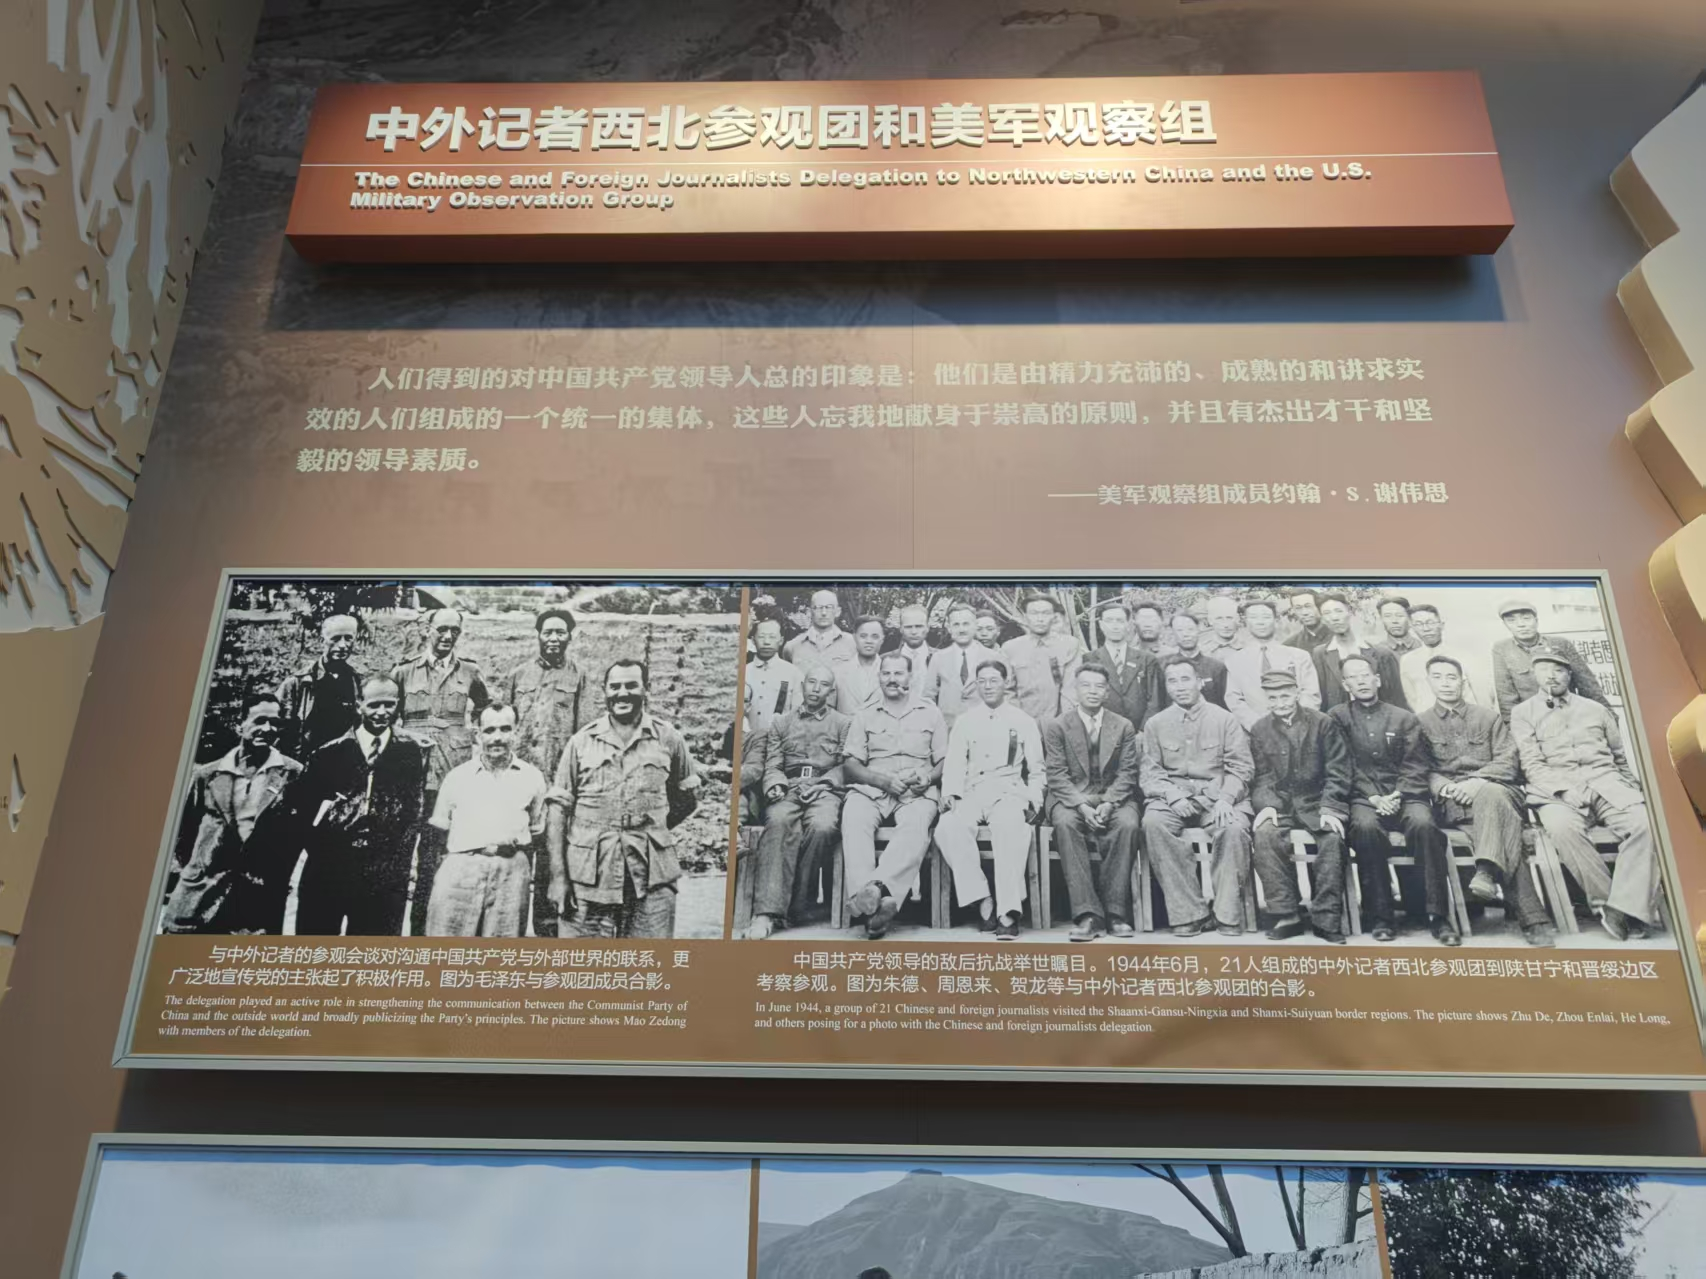
\includegraphics[width=0.7\textwidth]{A (13).jpg}
\caption{中外记者西北参观团和美军观察组展区}
\end{figure}

展区还专门介绍了支援中国抗战的国际友人。埃德加·斯诺1936年在宋庆龄帮助下进入陕北苏区采访，和毛泽东结下深厚友谊，写下了《红星照耀中国》（又名《西行漫记》）。这本书向全世界真实介绍了红色中国，感召了大量爱国青年和国际友人来华支援抗战，白求恩大夫就是受这本书影响来到中国的。苏联摄影师罗曼·卡尔曼1939年从重庆赴延安，实地拍摄记录边区军民生活，称赞延安是一座青春之城。抗战期间，大量国际记者、医生、技术人员来到敌后根据地，用文字、影像、行动支持中国人民的反法西斯斗争。

\begin{figure}[H]
\centering
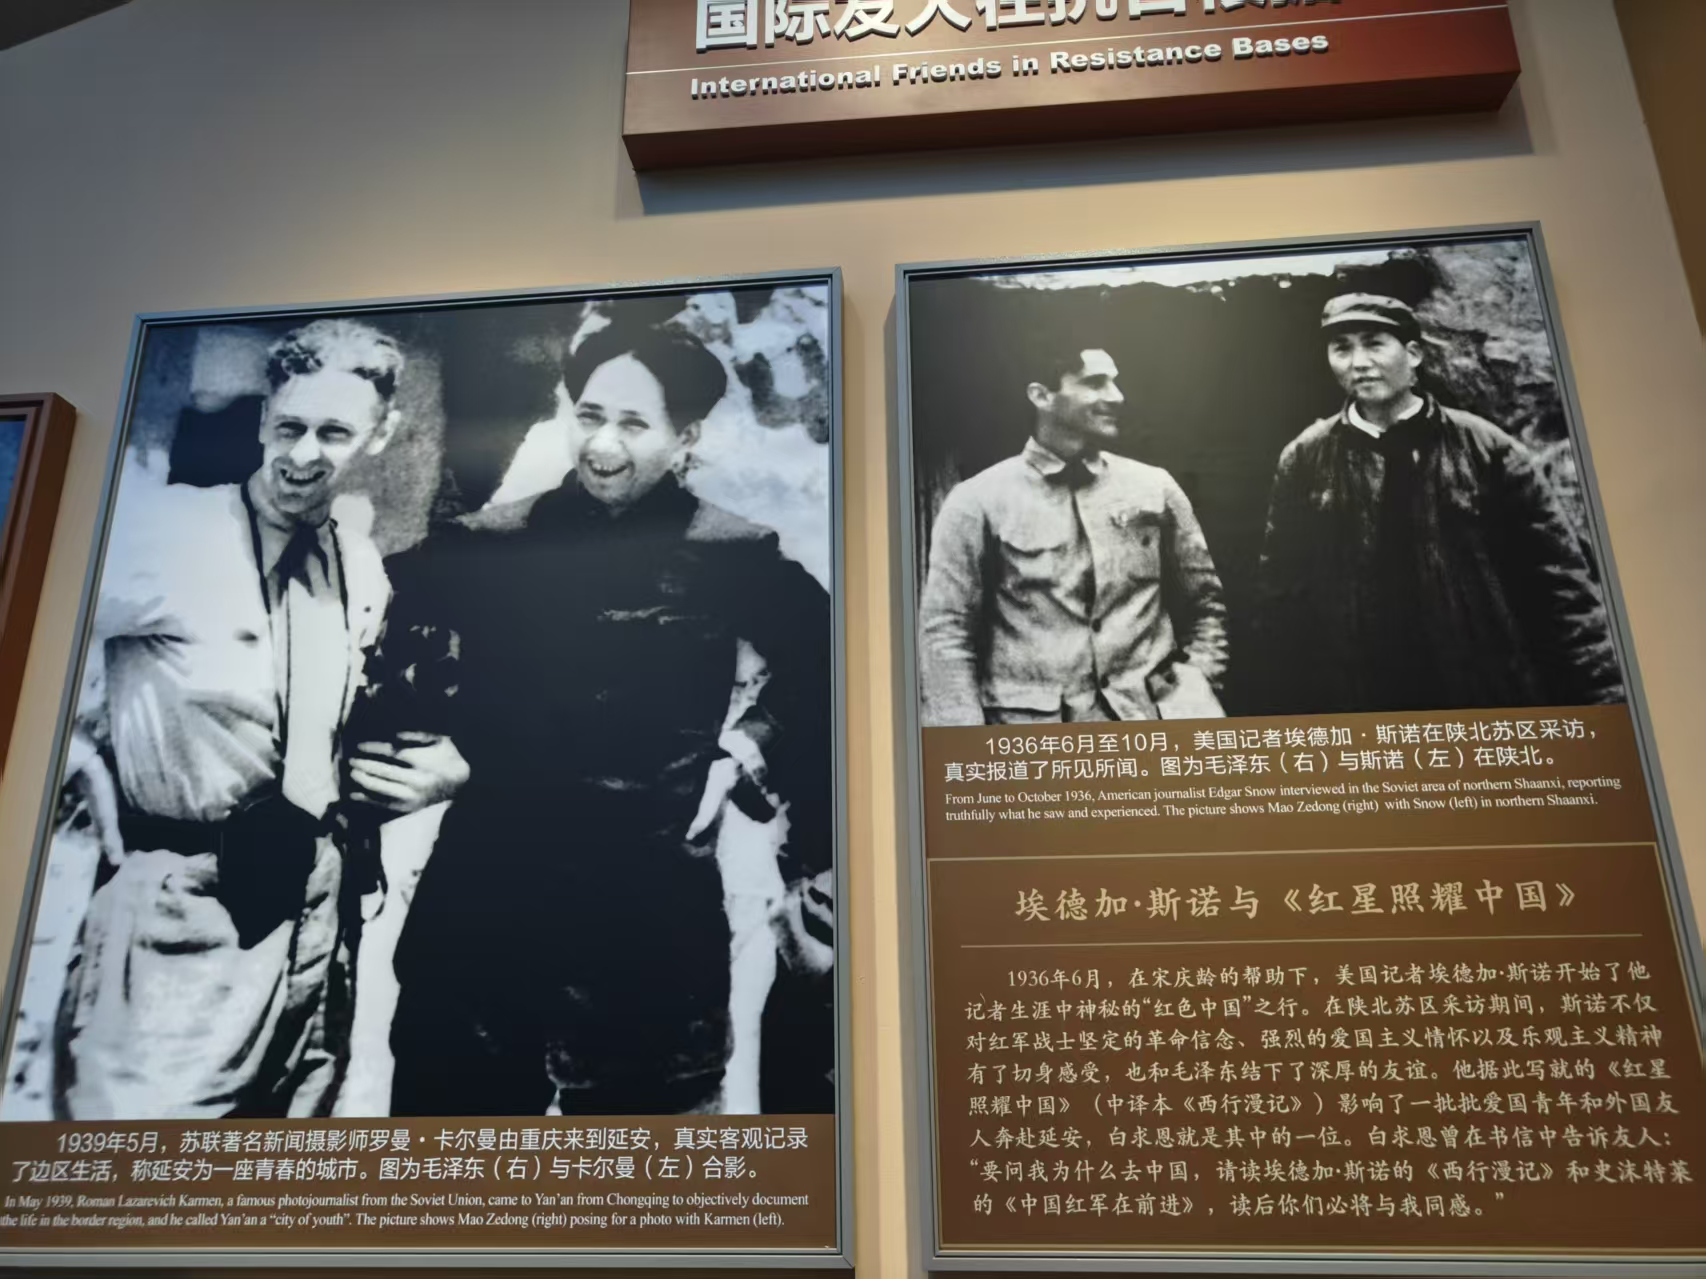
\includegraphics[width=0.7\textwidth]{A (14).jpg}
\caption{国际友人在抗日根据地展区}
\end{figure}

通过对第3展区的深入学习，我深刻认识到：中国共产党的坚强领导是抗战胜利的根本保证，人民群众是战争胜利的力量源泉。中国共产党不仅率先举起武装抗日的旗帜，而且制定了正确的战略方针，开辟了广阔的敌后战场，领导了伟大的人民战争。这一历史经验对于我们今天坚持党的领导、走群众路线具有重要启示意义。

\section*{\songti\zihao{-3}\textbf{五、第4展区：正面战场的英勇抗战——国共合作共御外侮}}

\subsection*{\songti\zihao{4}\textbf{（负责人：王冲）}}

作为第4展区的调研负责人，我系统学习了国民党军队在正面战场的抗战历程。这个展区全面展示了从卢沟桥事变到抗战中后期，国民党军队在正面战场与日军进行的一系列重大战役，体现了全民族抗战、国共合作的历史事实。

展区开篇即展示了七七事变的历史场景。1937年7月7日夜，日军在卢沟桥附近进行军事演习，借口一名士兵失踪，要求进入宛平城搜查，遭到中国守军拒绝后，悍然炮轰宛平城和卢沟桥。中国守军第29军奋起抵抗，打响了全民族抗战的第一枪。七七事变标志着中国人民抗日战争全面爆发，中华民族到了最危险的时候，全体中华儿女团结一致，共同抗击日本侵略者。

展区重点介绍了淞沪会战、太原会战、徐州会战、武汉会战、长沙会战等正面战场的重大战役。淞沪会战历时三个月，中国军队浴血奋战,粉碎了日军"三个月灭亡中国"的狂妄计划，但也付出了巨大牺牲。太原会战中，八路军配合国民党军队作战，取得了平型关大捷。徐州会战中的台儿庄大捷，是抗战初期正面战场取得的重大胜利，极大地鼓舞了全国人民的抗战信心。展区详细介绍了台儿庄战役的经过，展出了参战将领使用过的指挥刀、军服、勋章等珍贵文物，以及反映激烈战斗场面的历史照片。

展区特别介绍了为国捐躯的抗日将领。张自忠将军在枣宜会战中壮烈殉国，是抗战期间牺牲的最高级别将领；戴安澜将军率部远征缅甸，在抗击日军的战斗中英勇牺牲；左权将军是八路军在抗战中牺牲的最高级别将领。展区展示了这些抗日名将的生平事迹、遗物和后人的缅怀文字。他们的爱国主义精神和民族气节令人敬仰，他们用生命诠释了"天下兴亡、匹夫有责"的民族精神。

展区还介绍了正面战场与敌后战场的相互配合。全面抗战爆发后，国共两党实现第二次合作，建立抗日民族统一战线。国民党军队主要在正面战场抗击日军主力，八路军、新四军深入敌后开展游击战争，两个战场相互配合、相互支持，共同构成了中国抗战的完整图景。百团大战期间，八路军在华北地区对日军发动大规模攻势，有力地配合了正面战场的作战。

通过对第4展区的学习，我深刻认识到：抗日战争是全民族的战争，无论是共产党领导的军队还是国民党军队，无论是正面战场还是敌后战场，都为抗战胜利作出了贡献。只有全民族团结一致，才能战胜强大的敌人。这一历史经验告诉我们，在实现中华民族伟大复兴的新征程中，同样需要全体中华儿女团结奋斗。

\section*{\songti\zihao{-3}\textbf{六、第5展区：抗战胜利与历史启示——民族复兴的伟大转折}}

第5展区主要展示了抗日战争的最终胜利和深远影响，这是团队共同学习的重点内容。展区通过影像资料、历史文献和实物展示，呈现了从1944年中国军队发起战略反攻到1945年日本无条件投降的历史进程。

展区详细介绍了抗战后期中国战场的战略反攻。1944年，世界反法西斯战争进入决战阶段，中国战场也转入反攻。八路军、新四军在敌后战场发起局部反攻，收复大片失地。1945年春夏，解放区军民发起全面反攻，歼灭和瓦解大量日伪军。正面战场也展开反攻作战，收复失地。中国战场的胜利进展，有力地配合了盟军在太平洋战场和东南亚战场的作战。

展区重点展示了日本宣布无条件投降的历史时刻。1945年8月15日，日本天皇发表"终战诏书"，宣布无条件投降。9月2日，日本代表在停泊于东京湾的美国军舰"密苏里号"上签署投降书，标志着中国人民抗日战争暨世界反法西斯战争取得完全胜利。展区陈列的日本投降书复制件、受降仪式的历史照片、庆祝胜利的报纸等文物,让我们直观感受到胜利时刻全国人民的欢欣鼓舞。14年抗战，中国人民终于迎来了胜利的曙光。

展区特别设置了"抗战胜利的伟大意义"专题，系统阐述了抗战胜利的历史意义。第一，抗日战争是近代以来中国人民反抗外敌入侵第一次取得完全胜利的民族解放战争，洗刷了近代以来的民族耻辱，成为中华民族由衰败走向振兴的重大转折点。第二，中国人民抗日战争是世界反法西斯战争的重要组成部分，中国战场是世界反法西斯战争的东方主战场，中国人民为世界反法西斯战争胜利作出了巨大民族牺牲和重要历史贡献。第三，抗战胜利极大地提高了中国的国际地位，中国成为联合国安理会常任理事国，在战后国际秩序建立中发挥了重要作用。

展区还总结了抗战胜利的历史经验和启示。展板上习近平总书记在纪念中国人民抗日战争暨世界反法西斯战争胜利座谈会上的重要讲话摘录："中国人民抗日战争胜利，是近代以来中国抗击外敌入侵的第一次完全胜利。这一伟大胜利，彻底粉碎了日本军国主义殖民奴役中国的图谋，洗刷了近代以来中国抗击外来侵略屡战屡败的民族耻辱。"这段话深刻阐明了抗战胜利的历史意义。

通过学习，我们深刻领会到：抗战胜利的根本原因在于中国共产党发挥了中流砥柱作用，在于全民族的团结奋斗，在于以爱国主义为核心的伟大民族精神。伟大抗战精神——天下兴亡、匹夫有责的爱国情怀，视死如归、宁死不屈的民族气节，不畏强暴、血战到底的英雄气概，百折不挠、坚忍不拔的必胜信念——是中国人民弥足珍贵的精神财富，永远是激励中国人民克服一切艰难险阻、为实现中华民族伟大复兴而奋斗的强大精神动力。

\section*{\songti\zihao{-3}\textbf{七、实践收获与思考}}

\subsection*{\songti\zihao{4}\textbf{（一）个人收获与成长}}

通过本次暑期社会实践活动，团队每位成员都获得了深刻的思想教育和能力锻炼，实现了个人成长。

作为团队负责人王冲，在本次实践中不仅负责第4展区的调研学习，还要统筹整个团队的行程安排、纪律管理和安全保障。通过这次实践，我的组织协调能力、责任意识和领导力都得到了显著提升。同时，通过深入学习正面战场的抗战历史，我更加深刻地认识到国家统一、民族团结的重要性，也更加坚定了为国家富强、民族复兴而努力学习的决心。

安良玉同学负责第2展区日本侵华暴行板块的调研，面对大量触目惊心的历史资料，她始终保持认真严肃的态度，详细记录每一件展品、每一段历史。她表示，这次实践让她真正理解了"勿忘国耻"的深刻含义，也让她更加珍惜今天来之不易的和平生活。通过实践锻炼，她的历史分析能力、文字表达能力和情感共鸣能力都得到了提升。

刘佳鹏同学负责第3展区全民族抗战中流砥柱板块的学习，通过深入了解中国共产党在抗战中的光辉历程，他对党史有了更加系统深入的认识，更加坚定了听党话、跟党走的信念。他表示，《论持久战》等军事理论著作展现的战略智慧让他深受启发，今后要加强理论学习，提升科学思维能力。

\subsection*{\songti\zihao{4}\textbf{（二）团队协作与实践能力提升}}

本次实践活动采用团队协作模式，三位成员分工明确、相互配合，共同完成了参观学习、资料收集、照片拍摄、讨论交流、报告撰写等全部任务。通过团队协作，我们的沟通能力、协调能力、资料整理能力和文字表达能力都得到了显著提升。

在实践过程中，我们建立了有效的沟通机制。虽然每人负责不同的展区，但我们保持密切联系，及时分享学习心得和重要发现。在遇到问题时，大家集思广益、共同解决。这种团队协作精神不仅保证了实践活动的顺利进行，也增进了彼此的友谊和默契。

在资料收集和整理方面，我们各司其职、互相配合。文字记录人员认真记录展陈内容和解说词，摄影人员按照规定拍摄照片和视频，每个人都认真负责地完成自己的任务。实践结束后，我们汇总整理了所有调研笔记和影像资料，分类归档，为撰写实践报告提供了丰富的素材。

\subsection*{\songti\zihao{4}\textbf{（三）思想升华与责任担当}}

本次实践活动最大的收获是思想认识的升华。通过实地参观学习，我们深刻认识到历史的厚重和现实的责任，明确了新时代青年的使命担当。

我们深刻认识到，今天的和平生活来之不易，是无数革命先烈用鲜血和生命换来的。我们要倍加珍惜和平，坚决反对一切形式的侵略战争和霸权主义。同时，我们要保持清醒头脑，认识到国家安全面临的复杂挑战，自觉维护国家主权、安全和发展利益。

我们深刻认识到，中国共产党的领导是历史和人民的选择。正是在党的坚强领导下，中国人民才取得了抗战的伟大胜利，才实现了从站起来、富起来到强起来的伟大飞跃。在新时代，我们要坚定不移听党话、跟党走，为实现中华民族伟大复兴的中国梦贡献青春力量。

我们深刻认识到，青年一代有理想、有本领、有担当，国家就有前途，民族就有希望。在抗战时期,无数青年学生投笔从戎、奔赴前线，为民族独立和人民解放英勇奋斗。在新时代，我们同样要以天下为己任，把个人理想融入国家发展，在实现中国梦的生动实践中放飞青春梦想。

\section*{\songti\zihao{-3}\textbf{八、结语}}

本次中国人民抗日战争纪念馆暑期社会实践活动是一次深刻的爱国主义教育和红色基因传承活动。通过为期3小时的实地参观学习，我们系统了解了十四年抗战的历史进程，深切感受到革命先烈的英雄气概和民族精神，进一步增强了历史责任感和使命感。

在纪念馆外景的纪念碑前，镌刻着"1937.7.7"这个永远铭记的日子。七七事变标志着中国人民抗日战争全面爆发，中华民族开启了全民族抗战的伟大征程。纪念碑前摆放着群众敬献的白菊，表达着人们对革命先烈的深切缅怀。

\begin{figure}[H]
\centering
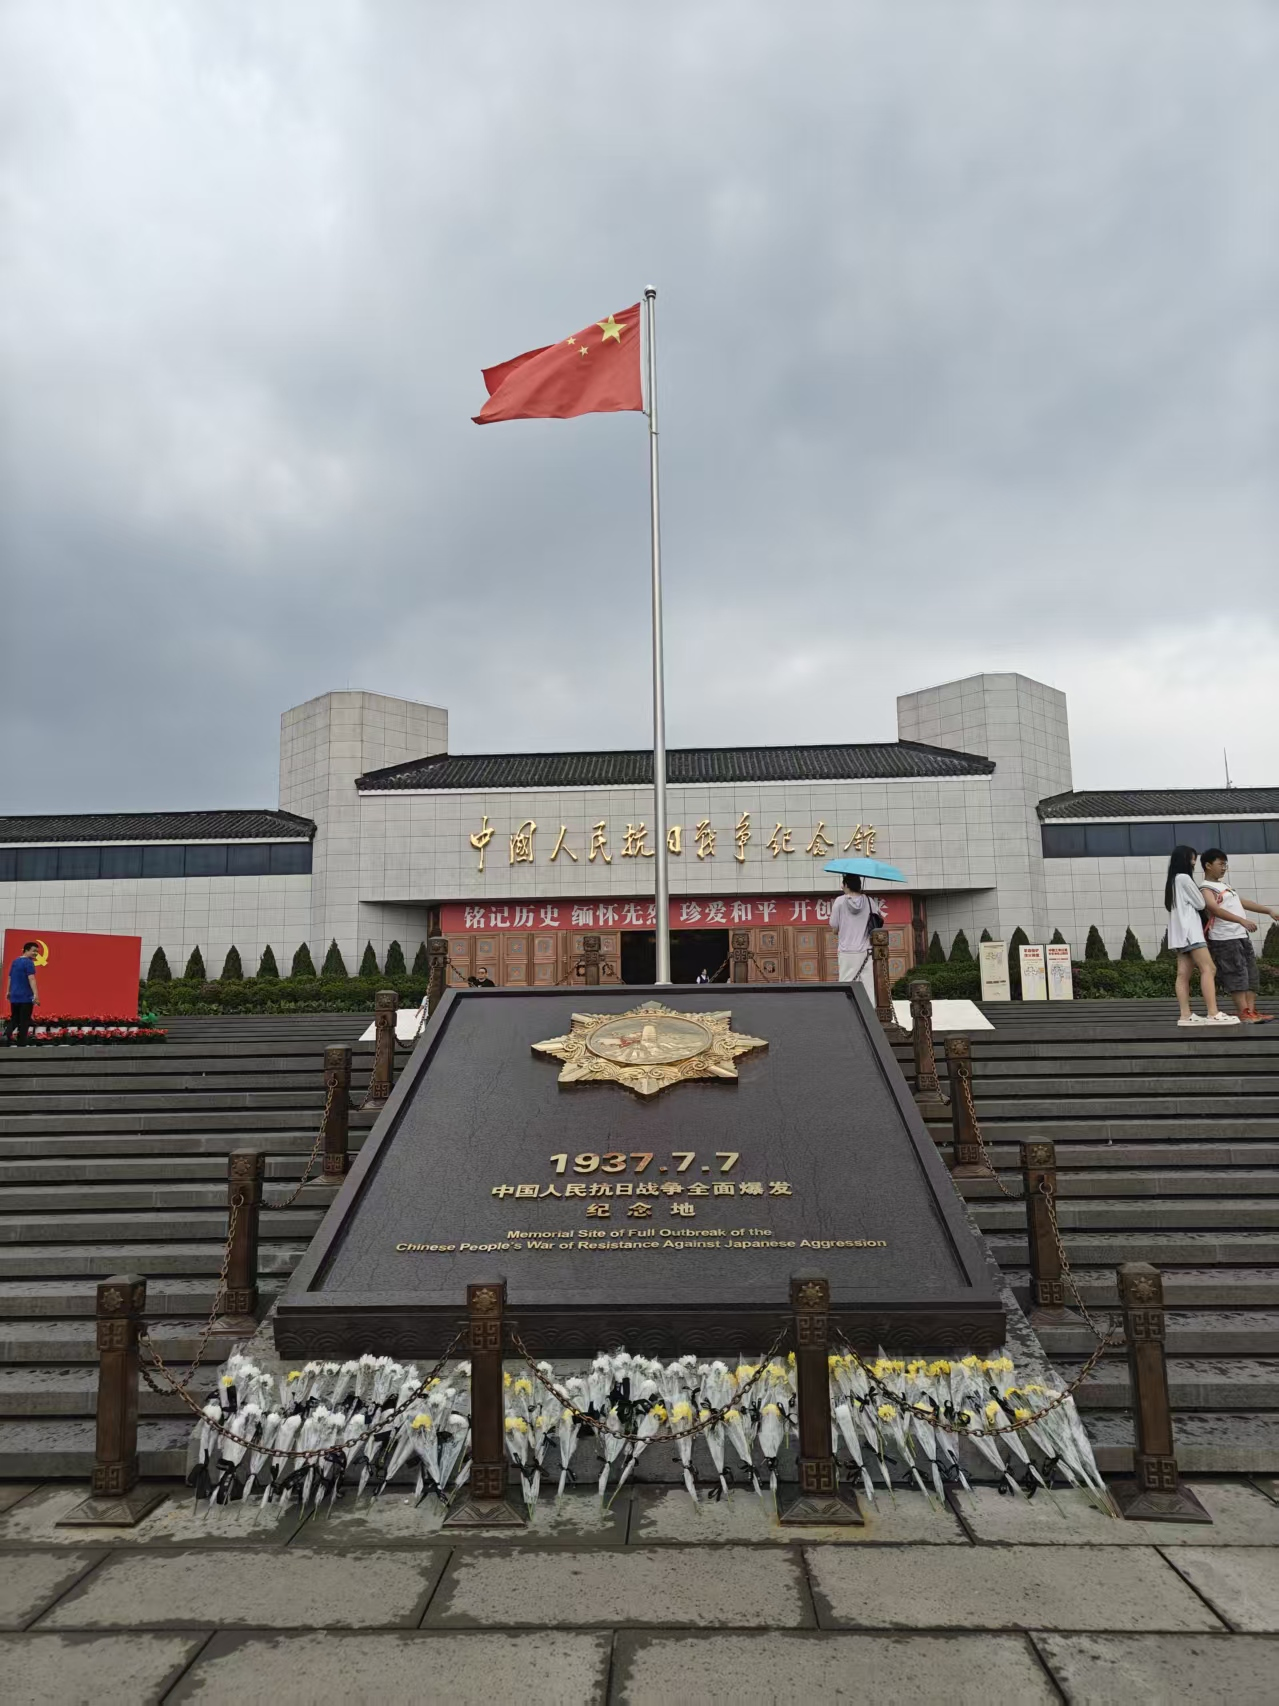
\includegraphics[width=0.7\textwidth]{A (11).jpg}
\caption{中国人民抗日战争纪念馆外景纪念碑}
\end{figure}

历史是最好的教科书，也是最好的清醒剂。抗日战争的历史告诉我们，落后就要挨打，发展才能自强。在实现中华民族伟大复兴的新征程上，我们要铭记历史、珍爱和平，大力弘扬伟大抗战精神，坚定理想信念，练就过硬本领，勇于创新创造，矢志艰苦奋斗，为实现中华民族伟大复兴的中国梦贡献青春力量。

正如习近平总书记所指出的："中国人民抗日战争胜利，是近代以来中国抗击外敌入侵的第一次完全胜利。这一伟大胜利，彻底粉碎了日本军国主义殖民奴役中国的图谋,洗刷了近代以来中国抗击外来侵略屡战屡败的民族耻辱。"我们要永远铭记这段历史，从中汲取前进的力量，为建设社会主义现代化强国、实现中华民族伟大复兴而不懈奋斗。

新时代赋予青年新使命，新征程呼唤青年新作为。我们将把本次实践活动的所学所思所悟转化为学习动力和行动自觉，在学习中增长知识、锤炼品格，在工作中增长才干、练就本领，在实践中认识国情、了解社会，努力成长为担当民族复兴大任的时代新人，为实现第二个百年奋斗目标、实现中华民族伟大复兴的中国梦贡献青春智慧和力量。

铭记烽火，赓续红色初心；不忘历史，勇担时代使命。这是我们这次实践活动最深刻的体会，也是我们对革命先烈最好的告慰。

\vspace{22pt}

\noindent\heiti\zihao{-4}\textbf{参考文献：}

\noindent\songti\zihao{5}
\setlength{\baselineskip}{22pt}
[1]中国人民抗日战争纪念馆.伟大胜利 历史贡献——纪念中国人民抗日战争暨世界反法西斯战争胜利70周年主题展览[M].北京：中国文史出版社,2015.

[2]习近平.在纪念中国人民抗日战争暨世界反法西斯战争胜利75周年座谈会上的讲话[N].人民日报,2020-09-04(02).

[3]中共中央党史研究室.中国共产党历史·第一卷（1921-1949）[M].北京：中共党史出版社,2011.

[4]军事科学院军事历史研究部.中国抗日战争史[M].北京：解放军出版社,2015.

[5]王建朗,黄克武.两岸新编中国近代史·抗日战争卷[M].北京：社会科学文献出版社,2016.

[6]中国人民抗日战争纪念馆.为了民族解放与世界和平——纪念中国人民抗日战争暨世界反法西斯战争胜利80周年主题展览[Z].北京,2025.

\vspace{22pt}

\begin{flushright}
\songti\zihao{5}
实践团队名称：赴北京市丰台区铭记烽火赓续红色初心调研实践团\\
团队成员：刘佳鹏\quad 安良玉\quad 王冲\\
指导教师：张天华\\
实践地点：中国人民抗日战争纪念馆\\
实践时间：2026年8月20日
\end{flushright}

\end{document}
